\documentclass{fdubeamer}

\usepackage{xcolor-material}
% This file contains shared definitions for main.tex and slide.tex.

% tikz
\usetikzlibrary{arrows.meta, calc, decorations.markings}
\tikzset{
  x = 1em,
  y = 1em,
  node font = \footnotesize,
  morphism box/.style = {draw, fill = white, anchor = base},
  vector box/.style = {thick, MaterialTeal, fill = MaterialTeal100},
  tensor box/.style = {thick, MaterialBlue, fill = MaterialBlue100},
  tensor leg/.style = {semithick, MaterialGrey},
  covered tensor leg/.style = {semithick, dashed, MaterialGrey300},
  ->-/.style = {
    decoration = {
      markings,
      mark = at position #1 with {\arrow{Stealth}},
    },
    postaction = {decorate},
  },
}
\ifdefined\tikzcdset
  \tikzcdset{
    arrow style = tikz,
    diagrams = {>=Stealth},
    arrows = {thin},
    labels = {font = \footnotesize},
  }
\fi
\newcommand{\tikzinput}[1]{\input{includes/tikz/#1.tex}}
\newcommand{\Vertex}[3]{
  \begin{tikzpicture}[baseline=0, thick]
    \draw (0,0) -- (90:1)  node [above] {$#1$}
          (0,0) -- (210:1) node [left]  {$#2$}
          (0,0) -- (330:1) node [right] {$#3$};
  \end{tikzpicture}
}
\newcommand{\Tetrahedron}[6]{
  \begin{tikzpicture}[baseline=1ex]
    \draw [covered tensor leg, MaterialGrey] (0,0) -- (3.2,0);
    \draw [tensor leg]
          (0,0) -- (2,2.5) -- (3.2,0) -- (2,-0.8) -- cycle
          (2,2.5) -- (2,-0.8);
    \draw (0.6, 1.7) node {$#1$}
          (3.2, 1.7) node {$#2$}
          (0.6,-0.9) node {$#3$}
          (3  ,-0.9) node {$#4$}
          (1.1, 0.5) node {$#5$}
          (2.4, 0.8) node {$#6$};
  \end{tikzpicture}
}
\newcommand{\Triangle}[6]{
  \begin{tikzpicture}[baseline=-0.5ex]
    \draw [tensor box]
          ( 90:1.5) -- (210:1.5) -- (330:1.5) -- cycle;
    \foreach \x in {90, 210, 330}
      \draw [tensor leg]
          (\x-40:1.7) .. controls (\x-20:0.8) and (\x+20:0.8) .. (\x+40:1.7)
          (\x-60:0.4) -- (\x-60:1.6);
    \draw ( 30:2) node {$#1$}
          (150:2) node {$#2$}
          (270:2) node {$#3$}
          ( 90:2) node {$#4$}
          (210:2) node {$#5$}
          (330:2) node {$#6$};
  \end{tikzpicture}
}
\newcommand{\VirutalHexagon}[1]{
  \begin{tikzpicture}[baseline=-0.2em]
    \draw [thick, dotted]
      (30:1.2) -- (90:1.2) -- (150:1.2) -- (210:1.2) -- (270:1.2) -- (330:1.2) -- cycle;
    #1;
  \end{tikzpicture}
}
\newcommand{\Fusion}[3]{
  \begin{tikzpicture}[baseline=-0.5em]
    \draw [thick, MaterialGrey]
      (0:0) -- ( 30:1.2)
      (0:0) -- (150:1.2)
      (0:0) -- (270:1.2);
    \draw
      ( 1.2,1.3) node {#1}
      (-1.2,1.3) node {#2}
      ( 0, -1.8) node {#3};
  \end{tikzpicture}
}

% Math commands
\newcommand{\dd}{\mathrm{d}}
\newcommand{\ee}{\mathrm{e}}
\newcommand{\ii}{\mathrm{i}}
\newcommand{\id}{\mathrm{id}}
\newcommand{\1}{\mathbb{1}}
\newcommand{\I}{\mathbb{I}}
\newcommand{\Z}{\mathbb{Z}}
\newcommand{\trans}{{\symsfup{T}}}
\newcommand{\bm}[1]{\symbf{#1}}
\newcommand{\ldual}[1]{{}^*\mspace{-2mu}#1}
\newcommand{\dv}[2]{\frac{\mathrm{d}#1}{\mathrm{d}#2}}
\newcommand{\pdv}[2]{\frac{\partial#1}{\partial#2}}
\renewcommand{\triangle}{\text{\scalebox{1.6}{$\bigtriangleup$}}}
\NewDocumentCommand{\bra}{som}{%
  \IfBooleanTF{#1}{\langle#3|}{%
    \IfValueTF{#2}{#2\langle#3#2|}{\left\langle#3\right|}}}
\NewDocumentCommand{\ket}{som}{%
  \IfBooleanTF{#1}{|#3\rangle}{%
    \IfValueTF{#2}{#2|#3#2\rangle}{\left|#3\right\rangle}}}
\NewDocumentCommand{\ev}{som}{%
  \IfBooleanTF{#1}{\langle#3\rangle}{%
    \IfValueTF{#2}{#2\langle#3#2\rangle}{\left\langle#3\right\rangle}}}
\DeclareMathOperator{\Hom}{Hom}
\DeclareMathOperator{\End}{End}
\DeclareMathOperator{\rank}{rank}
\DeclareMathOperator{\tr}{tr}
\DeclareMathOperator*{\argmin}{arg\,min}


\title{Aspects on Tensor Networks for Topological Orders}
\author{Xiangdong Zeng}
\institute{Supervisor: Prof.\ Ling-Yan Hung}
% \date{\today}

\begin{document}

\maketitle

\begin{frame}{Outline}

\begin{itemize}
  \item Motivation and background

    \begin{itemize}
      \item AdS/CFT correspondence
      \item Topological orders and category theory
      \item Tensor networks
    \end{itemize}

  \item Strange correlators and holographic tensor networks

    \begin{itemize}
      \item Tensor network representation of string-net model
      \item Strange correlators and MPO symmetries
      \item Construction of holographic tensor networks
      \item Operator pushing
    \end{itemize}

  \item Tensor network representations of Virasoro and Kac--Moody algebra

    \begin{itemize}
      \item Review of 2d CFT
      \item Basic construction
      \item Examples: Ising, dimer and Fibonacci models
    \end{itemize}
\end{itemize}

\end{frame}

\section{Motivation \& background}

\begin{frame}{Motivation: AdS/CFT correspondence}

\begin{columns}[c]

  \column{0.6\textwidth}

    \begin{itemize}
      \item Duality between a gravity theory in AdS\textsubscript{\textit{d}+1} spacetime (bulk)and a CFT\textsubscript{\textit{d}+1} (boundary)
      \item AdS/CFT dictionary: $Z_{\mathrm{CFT}}=Z_{\mathrm{bulk}}$
      \item Ryu--Takayanagi formula:

        \begin{itemize}
          \item $S_A = \operatorname{area}(\gamma_A) / 4G^{(d+1)}$
          \item Entanglement is geometry
        \end{itemize}

      \item AdS/CFT and machine learning

        \begin{itemize}
          \item Mapping to Boltzmann machine
          \item CNN as RG flow
        \end{itemize}

      \item \textit{p}-adic AdS/CFT and Einstein equation
    \end{itemize}

  \column{0.4\textwidth}

    \centering
    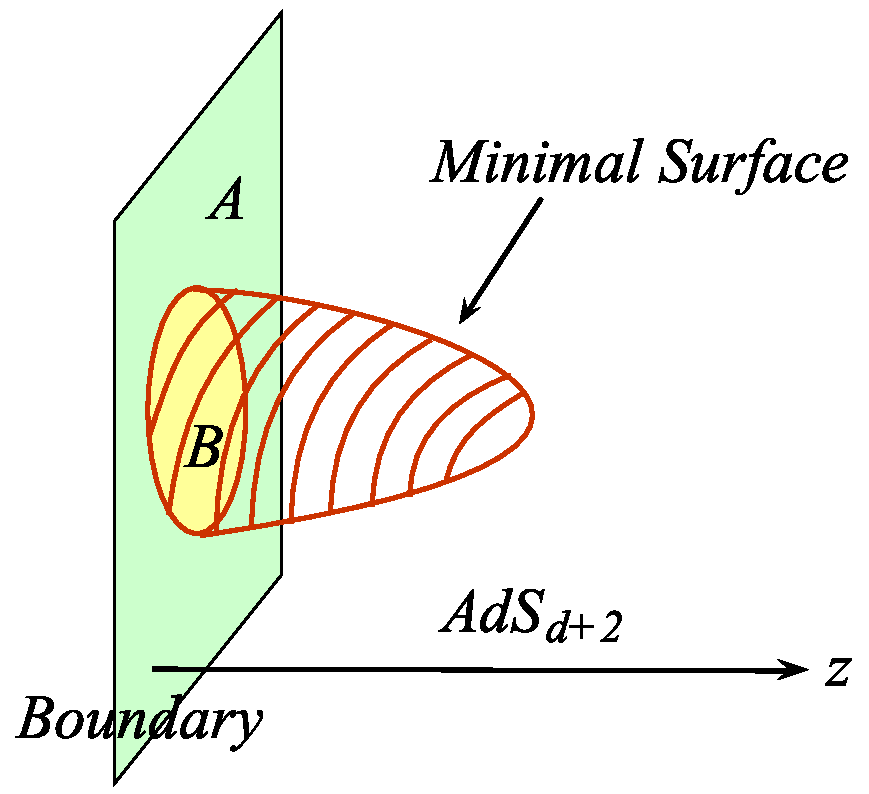
\includegraphics[width=0.8\textwidth]{images/rt-formula.pdf}

\end{columns}

\footnotetext{Image credit: \citet{nishioka2009holographic}}

\end{frame}

\begin{frame}{Topological orders}

\begin{itemize}
  \item Novel phases of matter beyond Landau's theory

    \begin{itemize}
      \item Fractional quantum Hall effect
      \item High temperature superconductivity
    \end{itemize}

  \item Fundamental properties:

    \begin{itemize}
      \item Ground state degeneracy
      \item Non-abelian geometric phase
    \end{itemize}

  \item Microscopic origin:

    \begin{itemize}
      \item Long-range entanglement
      \item Local unitary transformation
    \end{itemize}

  \item Applications: fault-tolerant quantum computation
  \item Mathematical framework: modular tensor categories (fusion categories)
\end{itemize}

\end{frame}

\begin{frame}{Tensor \& fusion categories}

\begin{itemize}
  \item Tensor product: $\otimes$

    \begin{itemize}
      \item Associativity: $(a\otimes b)\otimes c=a\otimes(b\otimes c)$
      \item Unit object: $\1\otimes a=a\otimes\1=a$
    \end{itemize}

  \item Simple objects and their fusion: $a\otimes b=\bigoplus_c N_{ab}^c c$

    \begin{itemize}
      \item Simple objects $a,b$: different types of anyon
      \item Fusion: can't be distinguished at long distance
      \item Fusion coefficients: $N_{ab}^c\in\Z^*$
      \item Quantum dimension $d_a$: max eigenvalue of matrix $(N_a)_{bc}=N_{ab}^c$
    \end{itemize}

  \item Examples:

    \begin{itemize}
      \item Decomposition of direct product of group representations
      \item Operator product expansion (OPE) in CFT
    \end{itemize}

  \item More structures: dual, braiding, ribbon, non-degeneracy, etc.
\end{itemize}

\end{frame}

\begin{frame}{Fusion diagrams}

\linespread{1.4}
\selectfont

\begin{columns}[c]

  \column{0.6\textwidth}

    \begin{itemize}
      \item Basis in vector space $\operatorname{Hom}_{\mathcal{C}}(a\otimes b,c)$:
            \tikzinput{category/fusion-tree-1}
      \item \textit{F}-move:
            $\tikzinput{category/f-symbol-1} = \sum_y \, \bigl[ F^{abc}_d \bigr]_{xy} \tikzinput{category/f-symbol-2}$
      \item Constraints: pentagon equations
      \item Bubble removal: \\
            \mbox{\qquad} $\tikzinput{category/loop-removal}$
    \end{itemize}

  \column{0.4\textwidth}

    \centering
    \tikzinput{category/f-symbols-pentagon-equation-narrow}

\end{columns}

\end{frame}

\begin{frame}{Examples of fusion categories}

\linespread{1.4}
\selectfont

\begin{itemize}
  \item Fibonacci

    \begin{itemize}
      \item Anyon types: $\{\1, \tau\}$
      \item Fusion rules: $\tau\otimes\tau=\1\oplus\tau$
      \item Quantum dimensions: $d_{\1}=1, \, d_\tau=\varphi$
      \item \textit{F}-symbols:
        $
          [F^{\tau\tau\tau}_\tau]_{ij} = \frac{1}{\varphi} \Bigl(\begin{smallmatrix} 1 & \sqrt\varphi \\ \sqrt\varphi & -1 \end{smallmatrix}\Bigr), \,
          i,j \in \{\1, \tau\}
        $
    \end{itemize}

  \item Ising

    \begin{itemize}
      \item Anyon types: $\{\1, \sigma, \psi\}$
      \item Fusion rules: $\psi\otimes\psi=\1, \, \sigma\otimes\sigma=\1\oplus\psi, \, \psi\otimes\sigma=\sigma$
      \item Quantum dimensions: $d_{\1}=d_\psi=1, \, d_\sigma=\sqrt2$
      \item \textit{F}-symbols:
        $
          [F^{\psi\sigma\psi}_\sigma]_{\sigma\sigma} = [F^{\sigma\psi\sigma}_\psi]_{\sigma\sigma} = -1, \,
          [F^{\sigma\sigma\sigma}_\sigma]_{ij} = -\frac{1}{\sqrt2} \Bigl(\begin{smallmatrix} 1 & 1 \\[0.5ex] 1 & -1 \end{smallmatrix}\Bigr), \,
          i,j \in \{\1, \psi\}
        $
    \end{itemize}
\end{itemize}

\end{frame}

\begin{frame}{String-net model}

\begin{itemize}
  \item Input data

    \begin{itemize}
      \item Trivalent lattice (e.g.\ honeycomb)
      \item Superselection sector (edge): simple objects
      \item Branching rules (vertex): fusion rules
    \end{itemize}

  \item Hamiltonian: $H = -\sum_v A_v - \sum_p B_p$

    \begin{itemize}
      \item Electric charge:
        $A_v \, \ket[\Bigg]{\tikzinput{string-net/fusion-2}} = \delta_{ijk} \, \ket[\Bigg]{\tikzinput{string-net/fusion-2}}$
      \item Magnetic flux:
        $B_p = \sum_{s=0}^N \frac{d_s}{D^2} B_p^s \, , \quad D = \sqrt{\sum_{s=0}^N d_s^2}$ \\
        $
            \phantom{\text{Magnetic flux:~}}
            B_p^s \, \ket[\Bigg]{\def\Prime{}\tikzinput{string-net/hexagon}}
          = \sum_{m,\dots,r} B_{p,ghijkl}^{s,g'h'i'j'k'l'} \,
            \ket[\Bigg]{\def\Prime{'}\tikzinput{string-net/hexagon}}
        $
    \end{itemize}
\end{itemize}

\end{frame}

\begin{frame}{Tensor networks}

\begin{columns}[c]

  \column{0.6\textwidth}

    \begin{itemize}
      \item Tensor: a multi-dimensional array
      \item Contraction and decomposition (SVD)
      \item Why efficient?

        \begin{itemize}
          \item Only keep the relevant (i.e.\ entanglement) degrees of freedom
          \item Area-law: $S\sim\partial A$
        \end{itemize}

      \item Algorithms:

        \begin{itemize}
          \item MPS/MPO based: DMRG, TEBD, etc.

            \begin{itemize}
              \item 2d generalization: PEPS/PEPO
            \end{itemize}

          \item Coarse-graining: TRG, TNR, HOTRG, etc.
          \item MERA: holographic geometry
        \end{itemize}
    \end{itemize}

  \column{0.4\textwidth}

    \centering
    \tikzinput{tensor-network/tensor-networks}

\end{columns}

\footnotetext{Image credit: \citet{orus2019tensor} (with modification)}

\end{frame}

\section{Strange correlators \& \\ holographic tensor networks}

\begin{frame}{Tensor network representation of string-net model}

\begin{columns}[c]

  \column{0.5\textwidth}

    \begin{itemize}
      \item Construct ground state: is given by 

        \begin{itemize}
          \item Apply $B_p$ on vacuum state $\ket{\diameter}$
          \item Weighted by quantum dimensions
          \item Use \textit{F}-moves to simplify
        \end{itemize}

      \item PEPS structure:

        \begin{itemize}
          \item Virtual indices: summed over \\
            \mbox{\qquad} (outside two legs: $\alpha,\beta,\gamma$)
          \item Physical indices: left uncontracted
            \mbox{\qquad} (inner one leg: $i,j,k$)
        \end{itemize}

      \item Tetrahedral symmetry: $A_4$ group
    \end{itemize}

  \column{0.5\textwidth}

    \begin{center}
      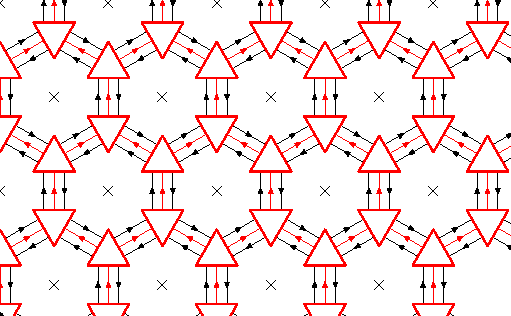
\includegraphics[width=0.7\textwidth]{images/string-net-peps.pdf}
      \scriptsize
      \setlength{\arraycolsep}{1.5pt}
      \tikzset{x=1em, y=1em, node font=\tiny}
      \begin{gather*}
          \Triangle jki\alpha\beta\gamma
        = \frac{1}{D} (d_i d_j d_k)^{-\frac14} (d_\alpha d_\beta d_\gamma)^{-\frac13}
          \Tetrahedron ik\gamma\alpha\beta j \\
          \bigl[ F^{abc}_d \bigr]_{xy}
        = \sqrt{d_x d_y} \begin{bmatrix} a & b & x\, \\ c & d & y\, \end{bmatrix}
        = \frac{1}{\sqrt{d_a d_b d_c d_d}} \, \Tetrahedron xbdyca
      \end{gather*}
    \end{center}
    \vspace*{-2em}

\end{columns}

\footnotetext{Image credit: \citet{buerschaper2009explicit}}

\end{frame}

\begin{frame}{Strange correlators}

\begin{itemize}
  \item Original definition: $C(r,r') = \langle\Omega|\phi(r)\phi(r')|\Psi\rangle / \langle\Omega|\Psi\rangle$

    \begin{itemize}
      \item $\ket{\Psi}$: a non-trivial short-range entangled (SPT) state
      \item $\ket{\Omega}$: a direct product state
    \end{itemize}

  \item In string-net model:

    \begin{itemize}
      \item $\ket{\Psi_\mathrm{SN}}$: PEPS wave function for string-net ground state
      \item $\ket{\Omega}$: some specific product state $\ket{\omega}^{\otimes N}$
      \item Partition function: $Z = \langle\Omega|\Psi_\mathrm{SN}\rangle = \tikzinput{strange-correlator}$

        \begin{itemize}
          \item Virtual indices (gray): summed over
          \item Physical indices (orange): fixed to some certain values (boundary conditions)
        \end{itemize}
    \end{itemize}
\end{itemize}

\end{frame}

\begin{frame}{Examples}

\begin{itemize}
  \item Fibonacci

    \begin{itemize}
      \item Boundary conditions: $\ket{\omega}=\ket{\tau}$
      \item Building blocks:
        \begingroup
          \scriptsize
          \tikzset{x=1em, y=1em, node font=\tiny}
          $
              \Triangle \tau\tau\tau\tau\tau\tau
            = \varphi^{\frac14} \bigl[ F^{\tau\tau\tau}_\tau \bigr]_{\tau\tau} = -\varphi^{-\frac34}, \,
              \Triangle \tau\tau\tau\1\tau\tau
            = \varphi^{\frac{7}{12}} \bigl[ F^{\tau\tau\tau}_\tau \bigr]_{\tau\1} = \varphi^{\frac{1}{12}}
          $
        \endgroup
    \end{itemize}

  \item Ising

    \begin{itemize}
      \item Boundary conditions: $\ket{\omega(\beta)} = \sqrt2 \, \bigl( \cosh\beta\ket{\1} + \sinh\beta\ket{\psi} \bigr)$
      \item Building blocks:
        \begingroup
          \scriptsize
          \tikzset{x=1em, y=1em, node font=\tiny}
          $
              A_{ijkl} = \tikzinput{ising/octagon} \enspace \text{where} \enspace
              i, j, k, l = \1 \text{ or } \psi, \enspace
              \tikzinput{ising/line-sigma} \, = \sigma, \enspace
              \tikzinput{ising/line-omega} \, = \omega
          $
        \endgroup
      \item Kramers--Wannier duality: shifted by 1/2 unit \textrightarrow{} $\beta_{\mathrm{c}}=\frac12\log(1+\sqrt{2})$
    \end{itemize}
\end{itemize}

\end{frame}

\begin{frame}{Application: calculation of central charge}

\begin{itemize}
  \item Use $A_{ijkl}$ as iMPO unit and perform iTEBD \textrightarrow{} $\{\Gamma,\lambda\}$
  \item Physical quantities:

    \begin{itemize}
      \item Correlation length: $\xi = -1 / \log|\lambda_2/\lambda_1|$
      \item Entanglement entropy: $S_{\!A} = \sum_i \lambda_i^2 \log \lambda_i^2$
    \end{itemize}

  \item Fit with $S_{\!A} \sim \frac{c}{6} \log \xi$ for different bond dimension $\chi$
\end{itemize}

\begin{center}
  \scriptsize
  \begin{tabular}{cc}
    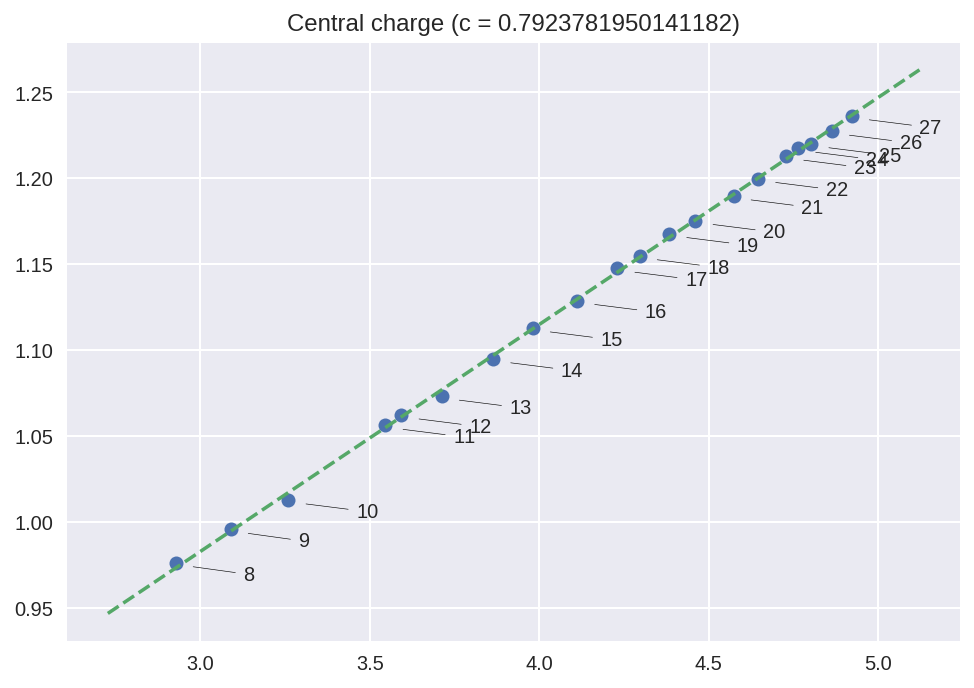
\includegraphics[width=0.3\textwidth]{images/fib-central-charge.png} &
    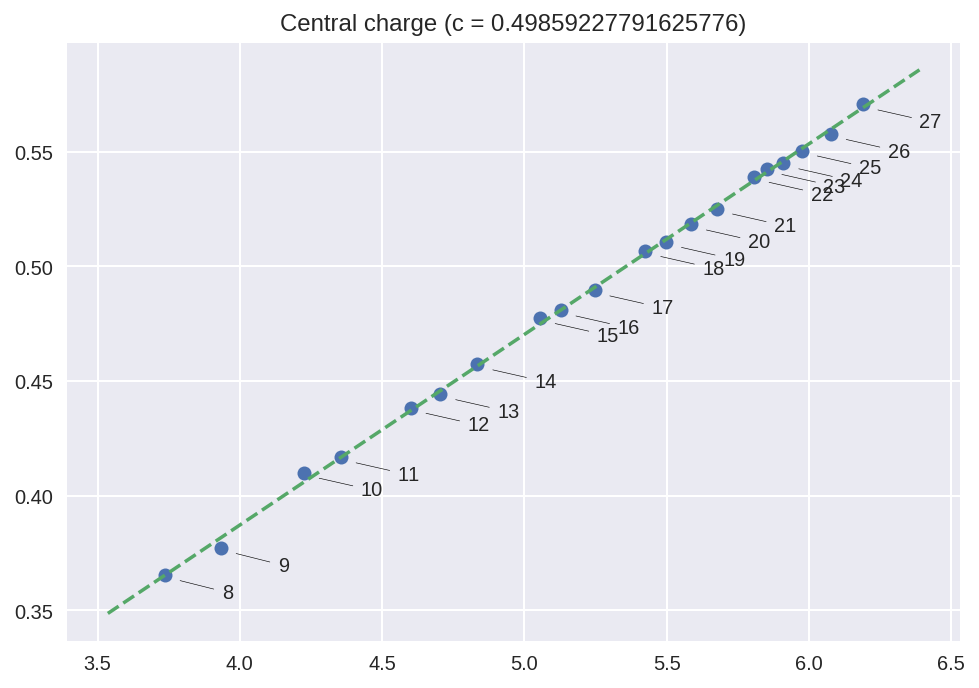
\includegraphics[width=0.3\textwidth]{images/ising-central-charge.png} \\
    Fibonacci: $c \simeq 0.792 \pm 0.004$ &
    Ising:     $c \simeq 0.499 \pm 0.004$
  \end{tabular}
\end{center}

\end{frame}

\begin{frame}{Holographic tensor networks in 2+1d}

\begin{itemize}
  \item $\ket{\Psi}$ is invariant under scaling transformation $\mathcal{H}_{\!\mathcal{C}}$
  \item Partition function is also invariant:
    $Z = \langle\Omega|\Psi\rangle = \langle\Omega|\exp(z\mathcal{H}_{\!\mathcal{C}})|\Psi\rangle$
  \item Eigenvalue problem:
    $\bra{\Omega}\exp(z\mathcal{H}_{\!\mathcal{C}}) = \bra{\Omega}FFF\cdots = \bra{\Omega}$

    \begin{itemize}
      \item Discrete Euclidean AdS space
    \end{itemize}
\end{itemize}

\centering
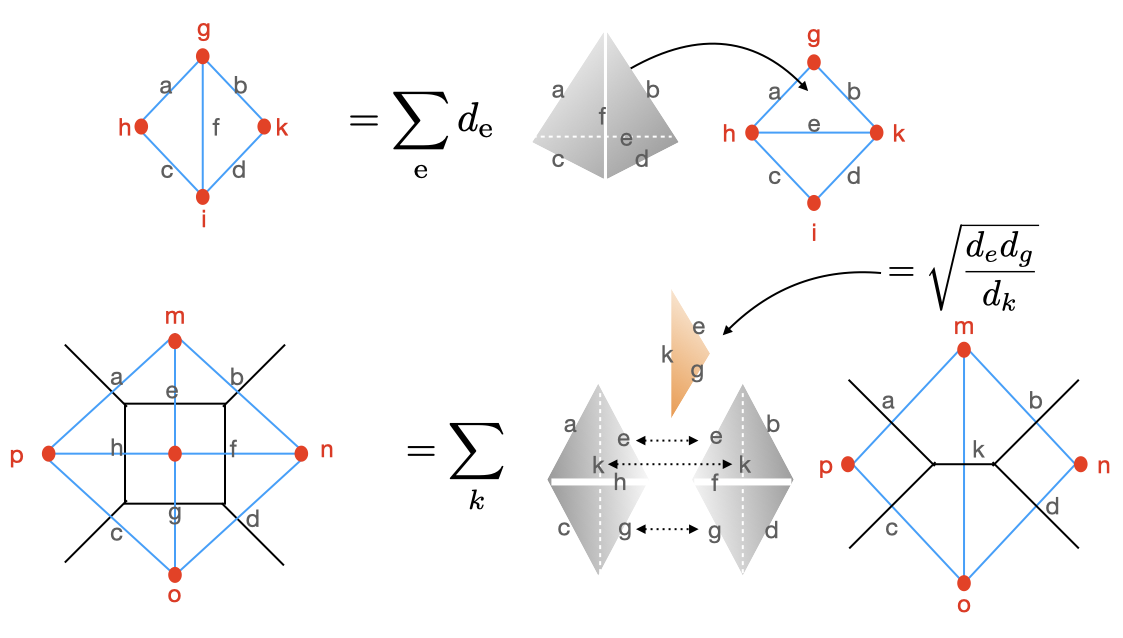
\includegraphics[width=0.5\textwidth]{images/holographic/tetrahedra-relations.png}

\footnotetext{Image credit: \citet{chen2022exact}}

\end{frame}

\begin{frame}{Details of RG procedure}

\begin{columns}[c]

  \column{0.5\textwidth}

    \begin{enumerate}
      \item PEPS tensor unit of $\bra{\Omega}$: $T^{a_1 a_2 a_3}_{I_1 I_2 I_3}$

        \begin{itemize}
          \item $a_i\in\mathcal{C}$: physical indices
          \item $I_i$: virtual indices (trivial at first)
        \end{itemize}

      \item Apply tetrahedra on surface to change its triangulation
      \item Use SVD to split coarse-grained tensor: $M^{acbd}_{ILJK}\to\tilde{T}^{akc}_{IHL}(k)\,\tilde{T}^{bdk}_{JHK}$

        \begin{itemize}
          \item $H$: new generated virtual index
          \item Bond dimension $\chi^2$ truncated to $\chi$
        \end{itemize}
    \end{enumerate}

  \column{0.5\textwidth}

    \centering
    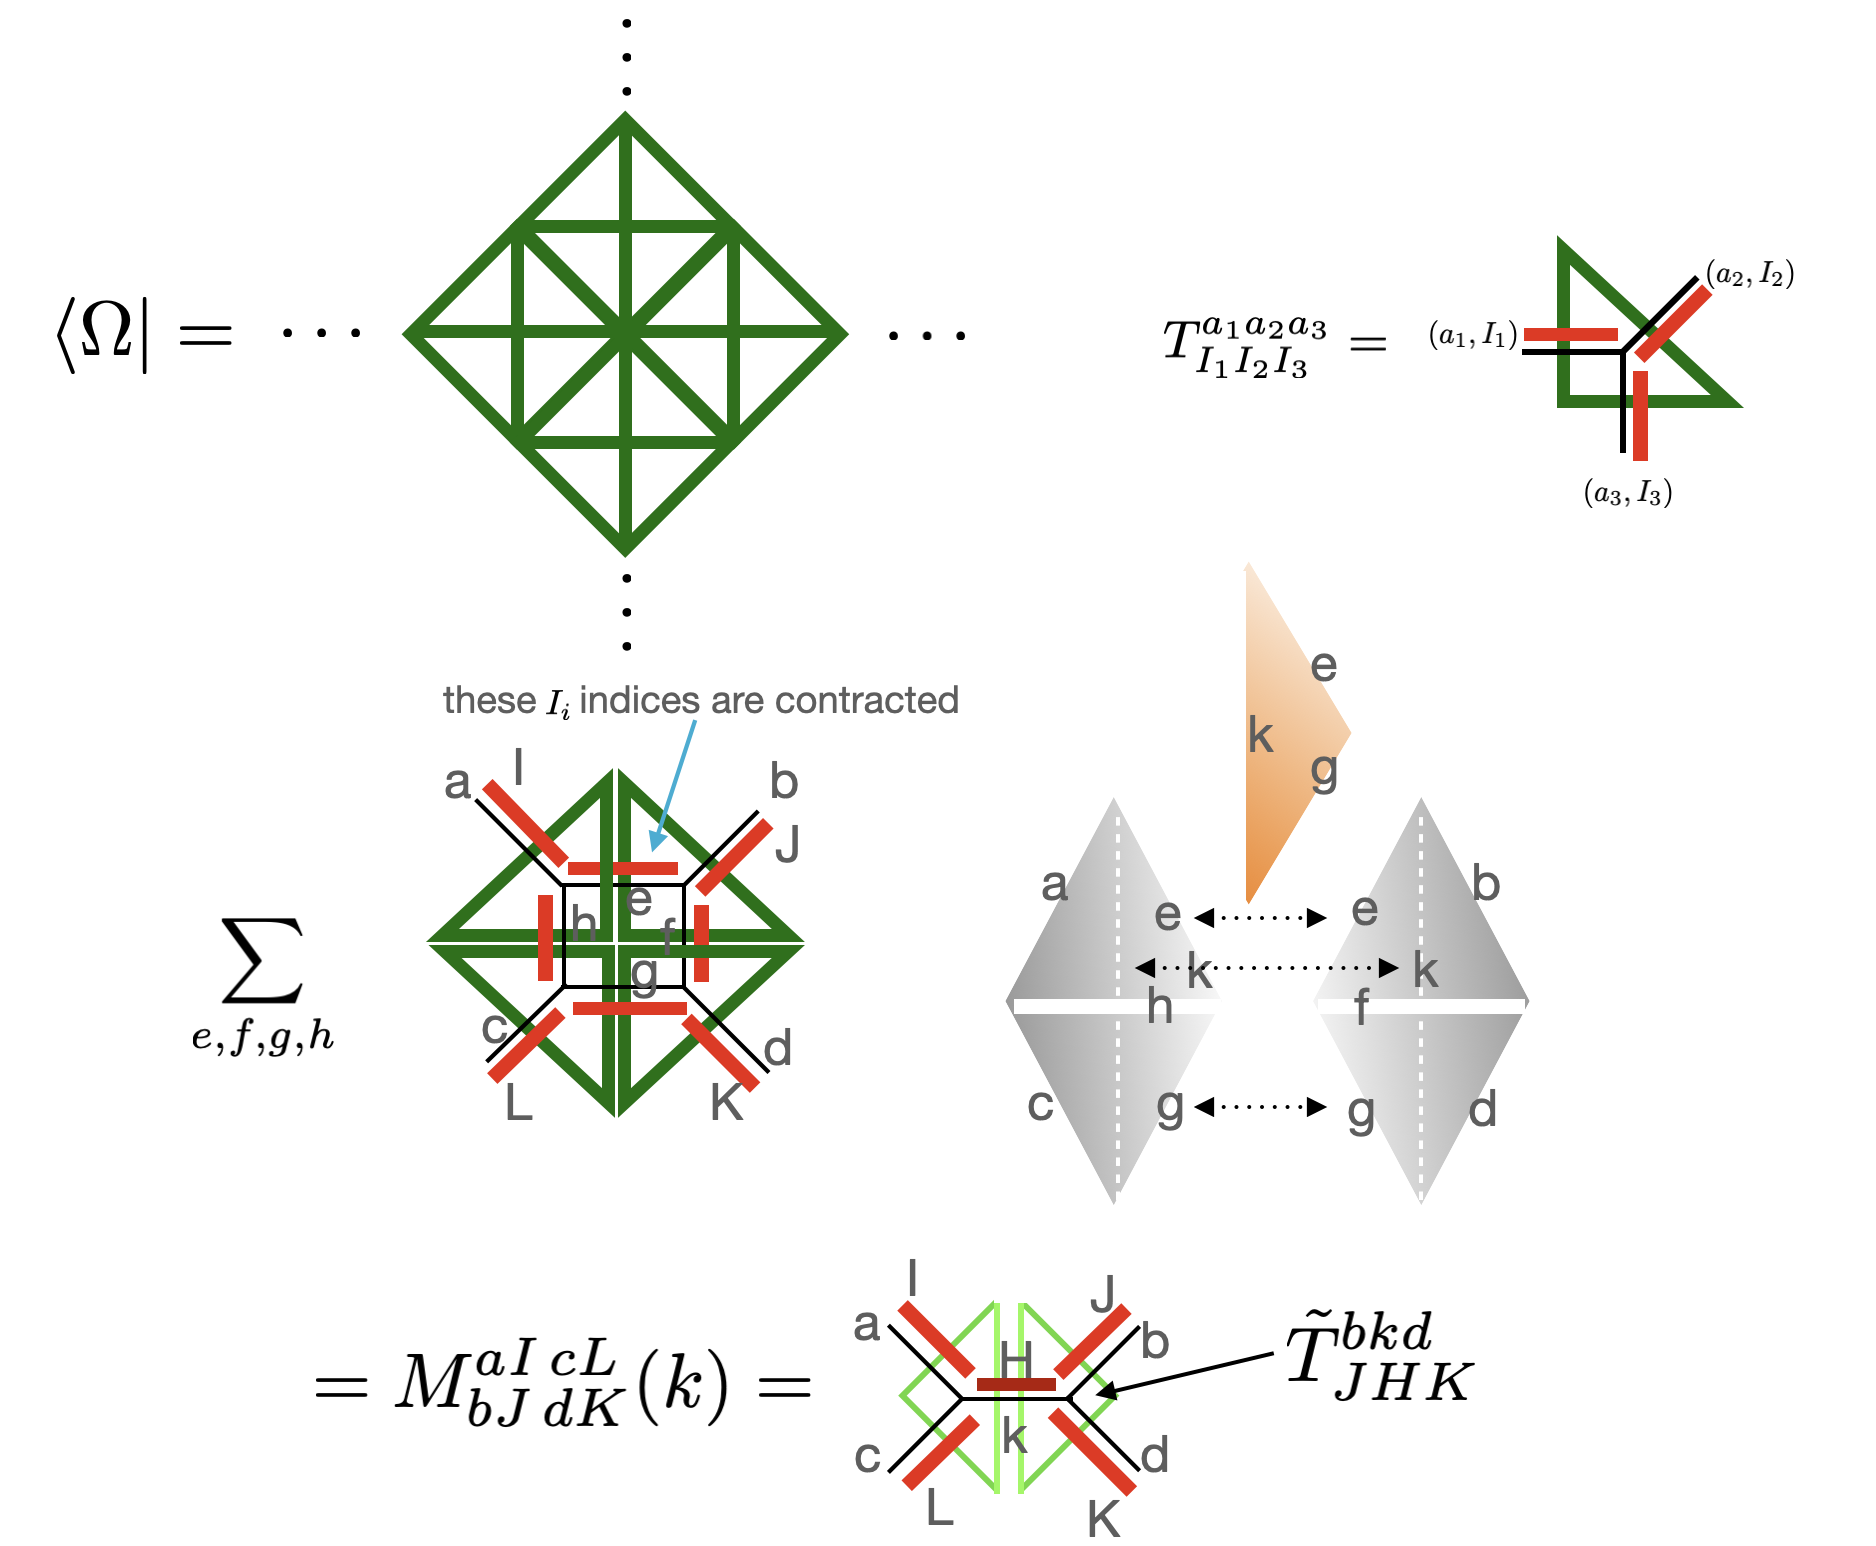
\includegraphics[width=0.85\textwidth]{images/holographic/rg-2+1d-blocking.png} \\[1ex]
    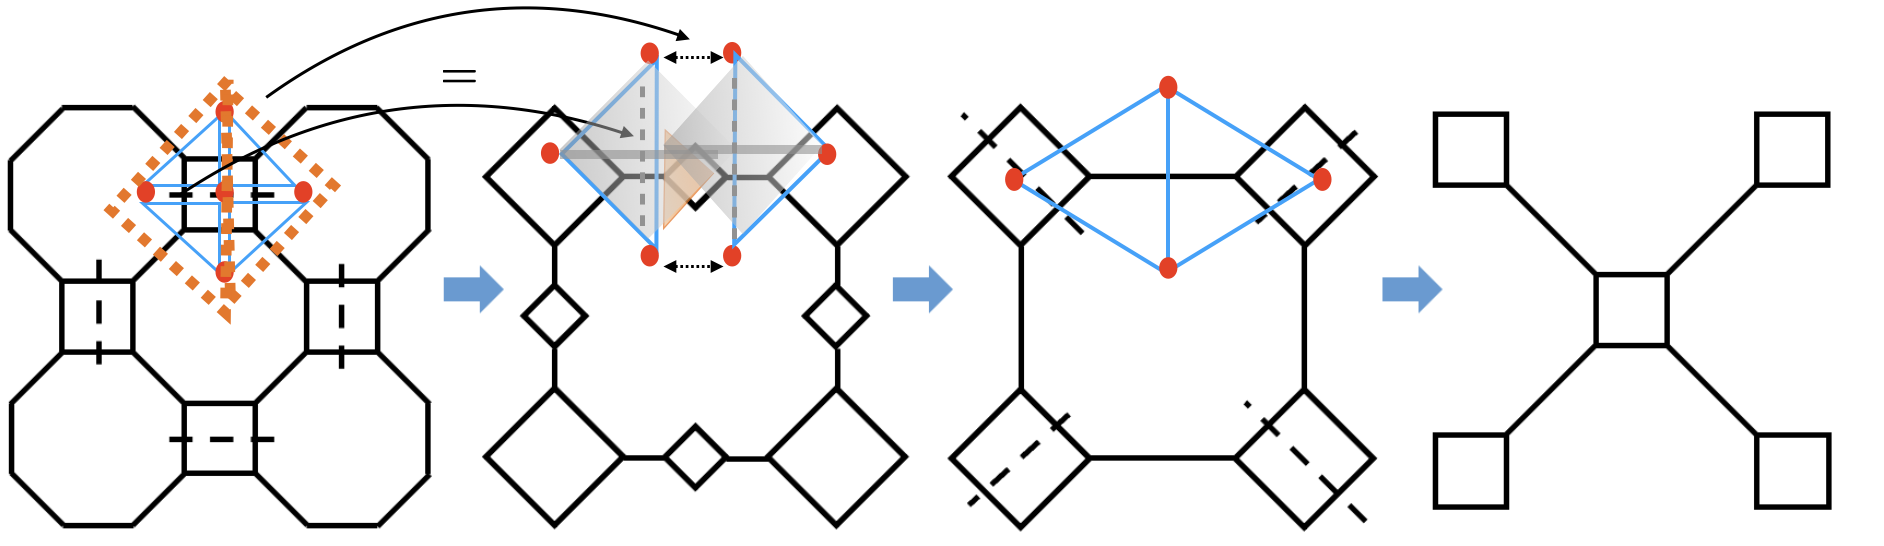
\includegraphics[width=0.75\textwidth]{images/holographic/rg-2+1d.png}

\end{columns}

\footnotetext{Image credit: \citet{chen2022exact}}

\end{frame}

% TODO: Fixed points & Frobenius algebra
\begin{frame}{Example: \texorpdfstring{$\mathcal{A}_{k+1}$}{𝒜ₖ₊₁} model [[TODO]]}

\begin{itemize}
  \item Boundary state: \\
    \begingroup
      \scriptsize
      \mbox{\qquad}
      $
        \bra{\Omega} = \sum_{\{a\}} \prod_{a_i} T^{a_1 a_2 a_3} \bra{\{a\}}, \quad 
        T^{a_1 a_2 a_3} = \begin{cases}
          1, & a_1 = a_3 = \frac12, \, a_2 = 0; \\
          r, & a_1 = a_3 = \frac12, \, a_2 = 1; \\
          0, & \mathrm{otherwise}
        \end{cases}
      $
    \endgroup

  \item Fixed points

    \begin{itemize}
      \item Classified by Frobenius algebra
      \item $T$ will eventually flow to a \emph{topological} fixed point for finite $\chi$
      \item \emph{Conformal} fixed point occurs when $T$ starts to converge to the topological one
    \end{itemize}
\end{itemize}

\end{frame}

\begin{frame}{Numerical results}

\begin{columns}[T]

  \column{0.5\textwidth}

    \begin{itemize}
      \item Fixed point tensor (at $\chi=1$)
      \item Small $r$

        \begin{itemize}
          \item Non-vanishing component: $T^{000}$
          \item Frobenius algebra: $\mathcal{A}_0=\{0\}$
        \end{itemize}

      \item Large $r$

        \begin{itemize}
          \item Non-vanishing component: \\
            \mbox{\quad} $T^{000}=T^{110}=T^{101}=T^{011}$
          \item Also exists $T^{111}$ at $k>2$
          \item Frobenius algebra: $\mathcal{A}_1=\{0,1\}$
          \item Ratio:
            $
              \dfrac{T^{000}}{T^{111}} \simeq \begin{cases}
                1.43463, & k = 3; \\[-0.5ex]
                1.18921, & k = 4
              \end{cases}
            $
        \end{itemize}
    \end{itemize}

  \column{0.5\textwidth}

    \vspace{-0.85em}
    \begin{itemize}
      \item Critical coupling:
        $r_{\!\mathrm{c}} = \frac{\sqrt[4]{2\cos\left(\frac{2\pi}{k+2}\right) + 1}}{\sqrt{2\cos\left(\frac{\pi}{k+2}\right) + 1}}$
      \item Recover to about 1 significant figure
    \end{itemize}

    \centering
    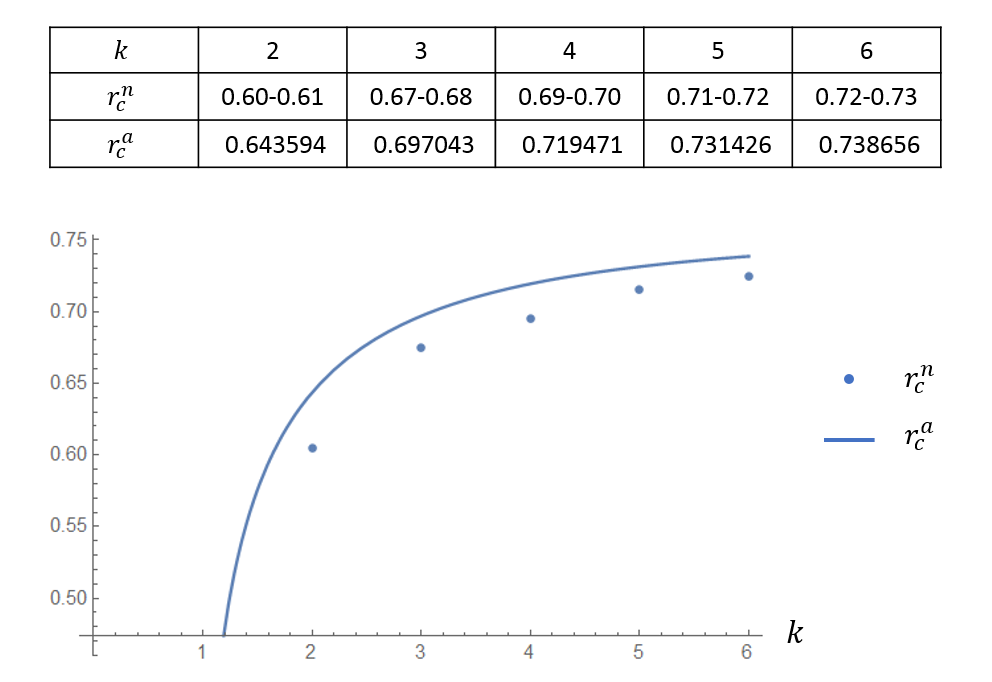
\includegraphics[width=0.9\textwidth]{images/holographic/a-k+1-coupling.png}

\end{columns}

\footnotetext{Image credit: \citet{chen2022exact}}

\end{frame}

\begin{frame}{Bulk-boundary propagators in 2d Ising model}

\begin{columns}[T]

  \column{0.6\textwidth}

    \begin{itemize}
      \item Correlation between bulk/boundary operators: \\[-2ex]
        \begingroup
          \small
          \mbox{\quad}
          $
            \begin{aligned}
              &\mathrel{\phantom{=}}
                 \ev[\big]{\mathcal{O}_{n=1}(0,0) \, \mathcal{O}_n(x,y)} \\
              &= \bigl\langle \Omega(T_{\Lambda_1}) \big|
                 \sigma^z(0,0) \, U^{n-1}(\mathcal{C}) \, \sigma^z(x,y) \, U^n(\mathcal{C}) \cdots
                 \big| \Psi \bigr\rangle \\
              &= \bigl\langle \Omega(T_{\Lambda_1}) \big|
                 \sigma^z(0,0) \, U^{n-1}(\mathcal{C}) \, \sigma^z(x,y)
                 \big| \Psi_{\Lambda_n} \bigr\rangle
            \end{aligned}
          $
        \endgroup
      \item AdS/CFT prediction: $\ev{\mathcal{O}_1 \, \mathcal{O}_n} \sim \left[ \frac{z}{x^2+z^2} \right]^\Delta$
      \item $\ev{\mathcal{O}_n\mathcal{O}_1} \sim z_n(x_n^2+1)$ plot indicates that the tensor network is holographic

        \begin{itemize}
          \item $\mathcal{O}_{1n}$: $\mathcal{O}_1$ pushed to $n$-th layer
          \item $z_n=(\sqrt{2})^{n-1}, \, x_n=x_1/z_n$
        \end{itemize}
    \end{itemize}

  \column{0.4\textwidth}

    \centering
    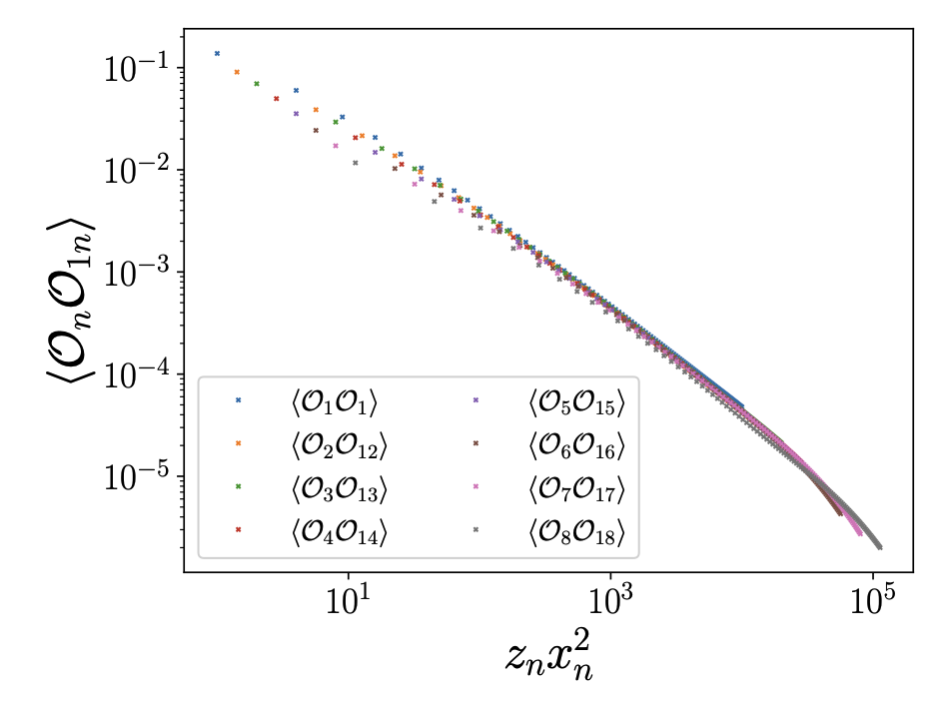
\includegraphics[width=0.8\textwidth]{images/holographic/bulk-boundary-propagator-1.png}
    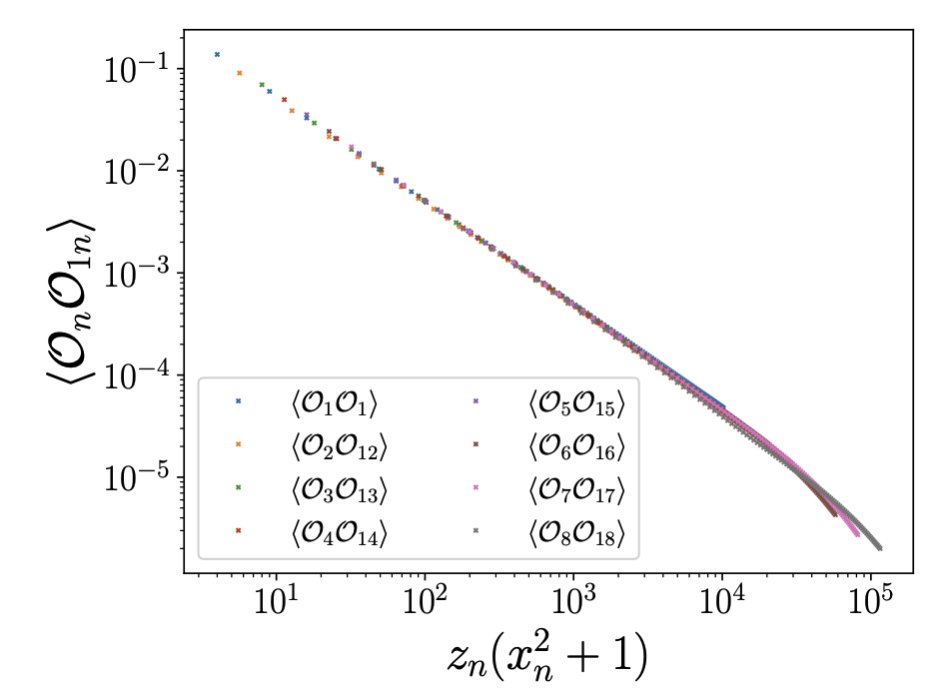
\includegraphics[width=0.8\textwidth]{images/holographic/bulk-boundary-propagator-2.png}
    \vspace{-0.5em}

\end{columns}

\footnotetext{Image credit: \citet{chen2022exact}}

\end{frame}

\begin{frame}{Generalization: 1+1d}

\begin{itemize}
  \item Dijkgraaf--Witten model characterized by group $G$
  \item Triangulation: $\alpha_2(g_1, g_2) \in H^2 \bigl(G, U(1)\bigr), \, g_1 \times g_2 = g_3$
  \item Associativity condition:

    \begin{itemize}
      \item $\alpha(g_1, g_2) \, \alpha(g_1 g_2, g_3) = \alpha(g_1, g_2 g_3) \, \alpha(g_2, g_3)$ \quad
        \begingroup
          \tikzset{x=0.6em, y=0.6em}
          \tikzinput{associativity-condition}
        \endgroup
      \item Convert the boundary circle with $2N$ edges to $N$ edges
    \end{itemize}
\end{itemize}

\begin{center}
  \scriptsize
  \tikzset{x=1em, y=1em, node font=\tiny}
  \tikzinput{rg-1+1d-disk}
\end{center}

\footnotetext{Image credit: \citet{chen2022exact}}

\end{frame}

\begin{frame}{Generalization: 3+1d}

\begin{itemize}
  \item 3+1d $\Z_2$ Dijkgraaf--Witten model (toric code) \textrightarrow{} 3d Ising model
  \item RG procedure:

    \begin{itemize}
      \item Smallest self-repeating unit: 2\texttimes 2\texttimes 2 cubes
      \item Eliminate edge centers \textrightarrow{} eliminate face centers \textrightarrow{} eliminate body centers
    \end{itemize}
\end{itemize}

\begin{columns}[c]

  \column{0.35\textwidth}

    \centering
    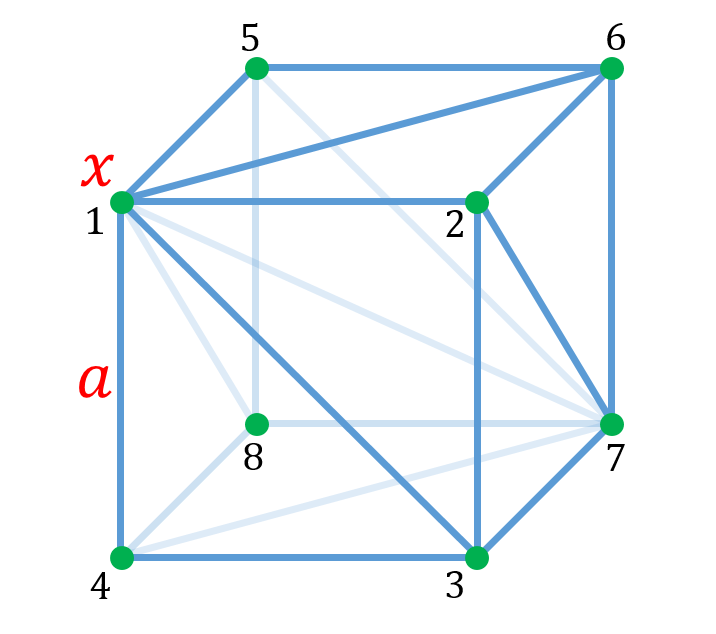
\includegraphics[width=0.4\textwidth]{images/holographic/3+1d-cube-1.png} \\[1ex]
    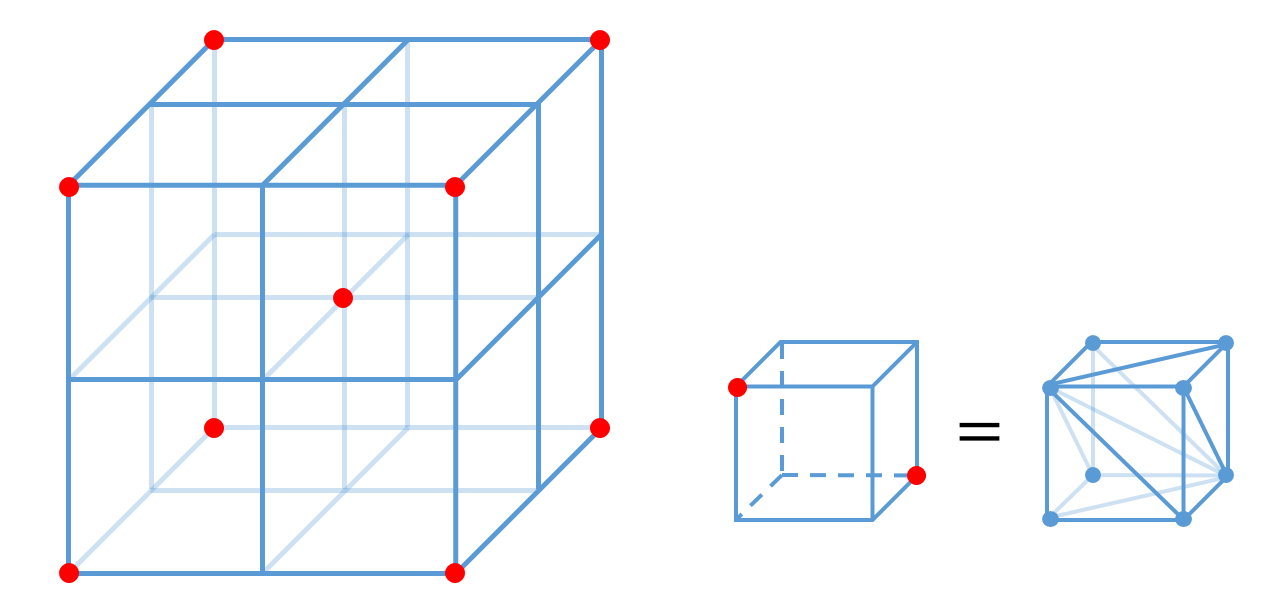
\includegraphics[width=0.7\textwidth]{images/holographic/3+1d-cube-2.png}
    \vspace{-1em}

  \column{0.65\textwidth}

    \centering
    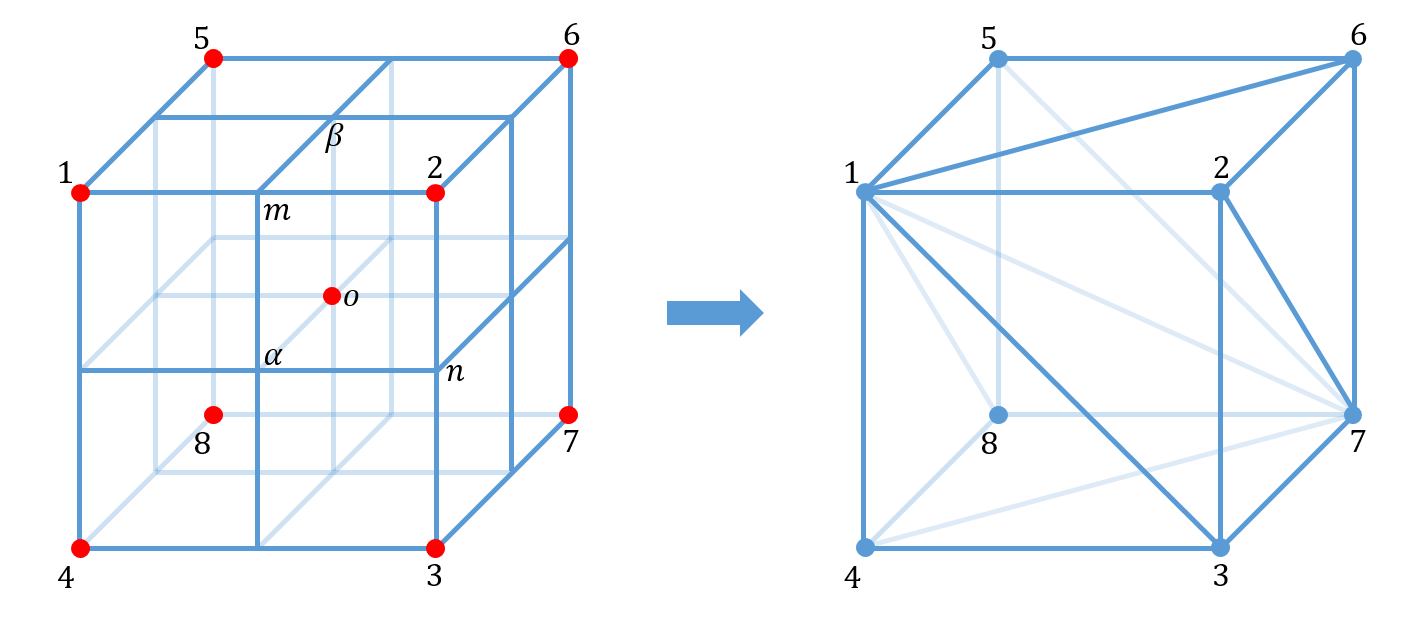
\includegraphics[width=0.45\textwidth]{images/holographic/rg-3+1d.png} \quad
    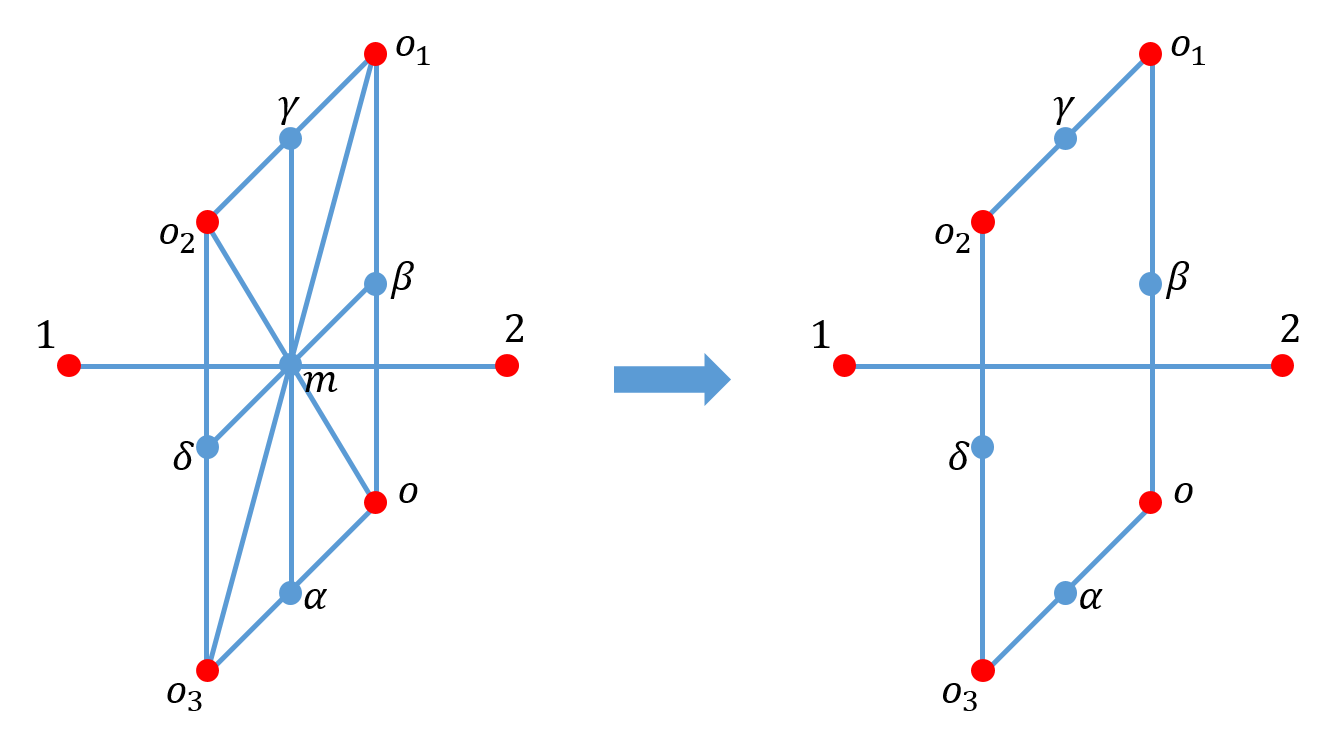
\includegraphics[width=0.45\textwidth]{images/holographic/rg-3+1d-step-1.png} \\
    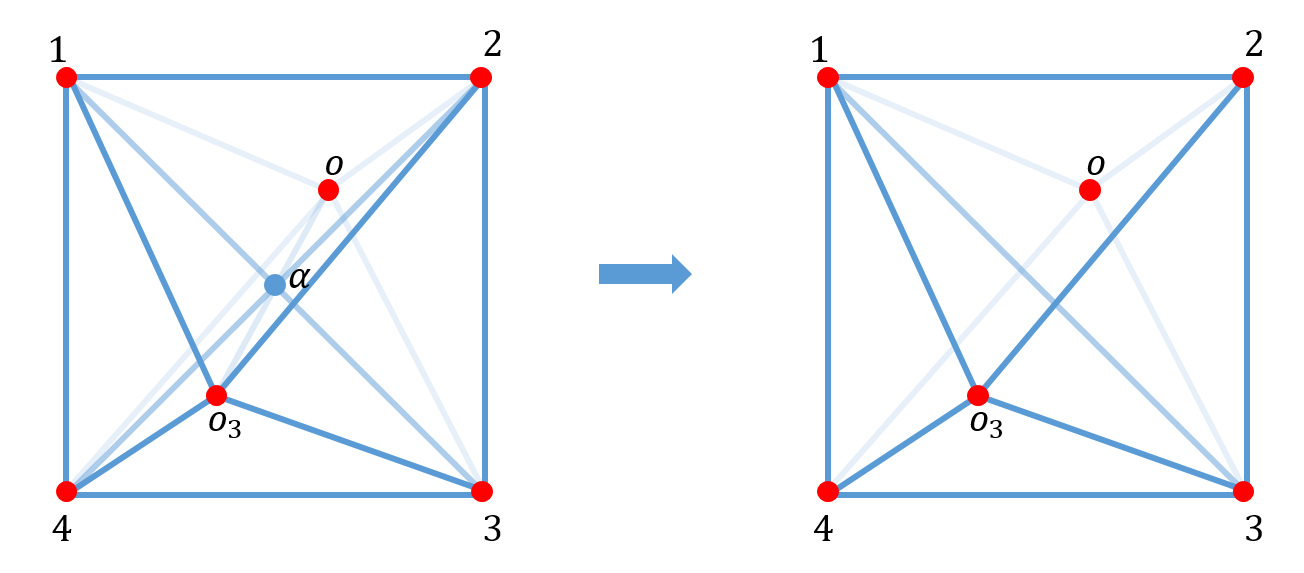
\includegraphics[width=0.45\textwidth]{images/holographic/rg-3+1d-step-2.png} \quad
    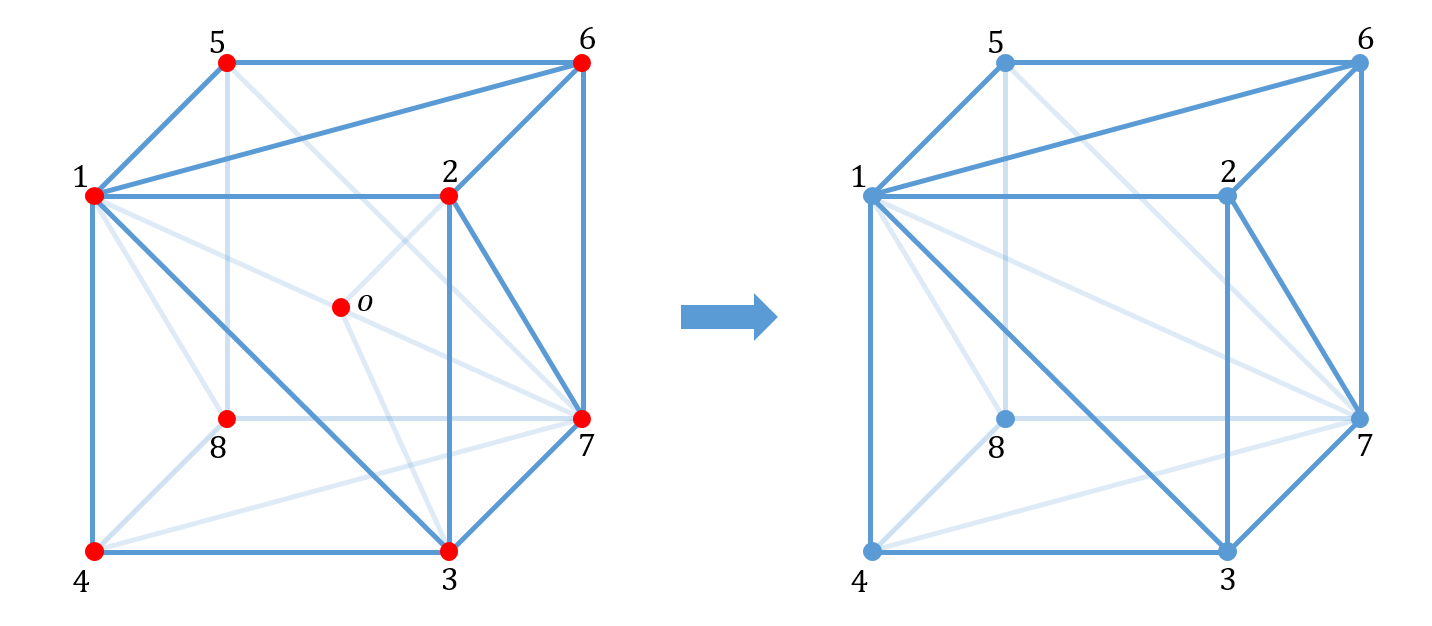
\includegraphics[width=0.45\textwidth]{images/holographic/rg-3+1d-step-3.png}

\end{columns}

\end{frame}

\begin{frame}{Bulk operator reconstruction \& operator pushing}

\begin{columns}[c]

  \column{0.65\textwidth}

    \begin{itemize}
      \item Generalized free fields

        \begin{itemize}
          \item Correlation functions are computed approximately by Wick contraction
          \item Can be decomposed as a sum of \emph{simple operators}
        \end{itemize}

      \item Operator pushing: $\mathcal{O} \bigl( \mathbb{V}^H \bigr) \cdot M = M \cdot \mathcal{O} \bigl( \mathbb{V}^K \bigr)$
        \begin{itemize}
          \item Bulk operator: $\mathcal{O} \bigl( \mathbb{V}^H \bigr)$ \\
            \mbox{\quad}
            $
              = \I_1 \otimes \cdots \otimes \I_{i-1} \otimes X_i \otimes \I_{i+1} \otimes \dots \otimes \I_{H}
            $
          \item Boundary operator: $\mathcal{O} \bigl( \mathbb{V}^K \bigr)$ \\
            \mbox{\quad}
            $
              = \sum_{i=1}^K \alpha_i \, \bigl(
                  \I_1 \otimes \cdots \otimes \I_{i-1} \otimes X_i \otimes \I_{i+1} \otimes \dots \otimes \I_{K}
                \bigr)
            $
        \end{itemize}
    \end{itemize}

  \column{0.35\textwidth}

    \begin{center}
      \scriptsize
      \tikzset{x=1em, y=1em, node font=\tiny}
      \tikzinput{operator-pushing/operator-pushing-narrow}
    \end{center}

\end{columns}

\footnotetext{Image credit: \citet{zeng2023bulk}}

\end{frame}

\begin{frame}{Operator pushing in 1+1d}

\linespread{1.4}
\selectfont

\begin{itemize}
  \item Find boundary operator $A$ for given bulk operator $B$, s.t. \\[0.8ex]
    \mbox{\qquad}
    \begingroup
      \scriptsize
      \tikzset{x=1em, y=1em, node font=\tiny}
      \tikzinput{operator-pushing/constraint-1+1d}
    \endgroup
    \quad\textrightarrow\quad
    $A_{(ij), (i'j')} M^{i'j'}_{ k} = M^{ij}_{k'} B_{k'k}$
  \item Generalized Pauli matrices: $\sigma_\mu \coloneq \sigma_{ns+t} = X^t Z^s$ where \\[1ex]
    \mbox{\qquad}
    $
      X = \left( \begin{smallmatrix}
        0      & 1      & 0      & \cdots & 0      \\
        0      & 0      & 1      & \cdots & 0      \\
        \vdots & \vdots & \vdots & \ddots & \vdots \\
        0      & 0      & 0      & \cdots & 1      \\
        1      & 0      & 0      & \cdots & 0
      \end{smallmatrix} \right)\!, \,
      Z = \left( \begin{smallmatrix}
        1      & 0      & \cdots & 0            & 0      \\
        0      & \omega & \cdots & 0            & 0      \\
        \vdots & \vdots & \ddots & \vdots       & \vdots \\
        0      & 0      & \cdots & \omega^{n-2} & 0      \\
        0      & 0      & \cdots & 0            & \omega^{n-1}
      \end{smallmatrix} \right)
    $
    \vspace{0.5ex}
  \item Constraint equations: $A_{(ij), (i'j')} \delta_{G(i',j'), k} = \delta_{G(i,j), k'} B_{k'k} = (\sigma_\mu)_{G(i,j), k}$

    \begin{itemize}
      \item One specific solution: $A^{(\mu)}_{(ij), (0j')} = (\sigma_\mu)_{G(i,j), j'}$
    \end{itemize}

  \item For simple form $A$: $\tilde{A}_{ii'} \delta_{G(i',j), k} - \sum_\mu \alpha_\mu (\sigma_\mu)_{G(i,j), k} \coloneq \tilde{M}(\cdots) = 0$
\end{itemize}

\end{frame}

\begin{frame}{Invitation: \texorpdfstring{$\Z_2$}{ℤ₂}}

\begin{itemize}
  \item Tensor unit:
    $
      M = \delta_{G(i,j),k} = \delta_{(i+j)\bmod 2,k} = \left( \begin{smallmatrix}
        1 & 0 \\  0 & 1 \\ 0 & 1 \\ 1 & 0 
      \end{smallmatrix} \right)
    $
  \item Null space:
    $
      \{ v^{(p)} \} = \left\{ \,
        \left( \begin{smallmatrix} 1 \\ 0 \\ 0 \\ -1 \end{smallmatrix} \right)\!, \,
        \left( \begin{smallmatrix} 0 \\ 1 \\ -1 \\ 0 \end{smallmatrix} \right) \,
      \right\}
      \implies
      A^* = \left( \begin{smallmatrix}
        \beta_{0,0} & \beta_{0,1} & -\beta_{0,1} & -\beta_{0,0} \\
        \beta_{1,0} & \beta_{1,1} & -\beta_{1,1} & -\beta_{1,0} \\
        \beta_{2,0} & \beta_{2,1} & -\beta_{2,1} & -\beta_{2,0} \\
        \beta_{3,0} & \beta_{3,1} & -\beta_{3,1} & -\beta_{3,0}
      \end{smallmatrix} \right)
    $
  \item Full solutions:
    $
      \left\{ \begin{aligned}
        & B = \I \implies A = A^* + \left( \begin{smallmatrix}
            1 & 0 & 0 & 0 \\ 0 & 1 & 0 & 0 \\ 0 & 1 & 0 & 0 \\ 1 & 0 & 0 & 0
        \end{smallmatrix} \right) \\
        & B = \sigma_x \implies A = A^* + \left( \begin{smallmatrix}
          0 & 1 & 0 & 0 \\ 1 & 0 & 0 & 0 \\ 1 & 0 & 0 & 0 \\ 0 & 1 & 0 & 0
        \end{smallmatrix} \right)
        \implies A = \I \otimes \sigma_x \text{ or } \sigma_x \otimes \I \\
        & B = \sigma_z \implies A = A^* + \left( \begin{smallmatrix}
          1 &  0 & 0 & 0 \\ 0 & -1 & 0 & 0 \\ 0 & -1 & 0 & 0 \\ 1 &  0 & 0 & 0
        \end{smallmatrix} \right) \\
        & B = -\ii\sigma_y \implies A = A^* + \left( \begin{smallmatrix}
          0 & -1 & 0 & 0 \\ 1 &  0 & 0 & 0 \\ 1 &  0 & 0 & 0 \\ 0 & -1 & 0 & 0
        \end{smallmatrix} \right)
      \end{aligned} \right.
    $
\end{itemize}

\end{frame}

\begin{frame}{Abelian example: \texorpdfstring{$\Z_n$}{ℤₙ}}

\linespread{1.4}
\selectfont

\begin{itemize}
  \item Fusion rules: $G(i,j) = (i+j)\bmod n$
  \item General solutions:

    \begin{itemize}
      \item General part:
        $
          A^* = \left( \begin{smallmatrix}
            \beta_{0,0} v^{(0)} + \dots + \beta_{0,n^2-n-1} v^{(n^2-n-1)} \\[0.5ex]
            \vdots \\
            \beta_{n^2-1,0} v^{(0)} + \dots + \beta_{n^2-1,n^2-n-1} v^{(n^2-n-1)}
          \end{smallmatrix} \right)
        $
      \item Specific part: $A^{(\mu)}_{(ij), (0j')} = (\sigma_\mu)_{(i+j)\bmod n, j'}$
    \end{itemize}

  \item Simple form solutions:

    \begin{itemize}
      \item $\operatorname{size}(\tilde{M})=n^3\times2n^2, \, \rank(\tilde{M})=2n^2-n$
      \item $n$ solutions: $\tilde{A}^{(k)}_{ii'} = (\sigma_k)_{ii'}, \, \alpha^{(k)}_\mu = \delta_{k\mu}$
      \item Generalized free fields $B=\sigma_k$ \textrightarrow{} $A=\sigma_k\otimes\I$ or $\I\otimes\sigma_k$
      \item Tensor network of $L$ layers: $A_L = \I^{\otimes L-l-1} \otimes \sigma_k \otimes \I^{\otimes l}$
    \end{itemize}
\end{itemize}

\end{frame}

\begin{frame}{Non-abelian example: \texorpdfstring{$S_3$}{𝑆₃}}

\begin{itemize}
  \item Group multiplication table:
    \begingroup
      \tiny
      \setlength{\arraycolsep}{4pt}
      $
        \begin{array}{c|cccccc}
          & g_0 & g_1 & g_2 & g_3 & g_4 & g_5 \\
          \hline
          g_0 & g_0 & g_1 & g_2 & g_3 & g_4 & g_5 \\
          g_1 & g_1 & g_0 & g_3 & g_2 & g_5 & g_4 \\
          g_2 & g_2 & g_4 & g_0 & g_5 & g_1 & g_3 \\
          g_3 & g_3 & g_5 & g_1 & g_4 & g_0 & g_2 \\
          g_4 & g_4 & g_2 & g_5 & g_0 & g_3 & g_1 \\
          g_5 & g_5 & g_3 & g_4 & g_1 & g_2 & g_0
        \end{array}
      $
    \endgroup
  \item Null space: spanned by $v^{(p)}=\bigl( \tilde{v}^{(p)}, \, \hat{v}^{(p)} \bigr)^\trans$

    \begin{itemize}
      \item $\tilde{v}^{(1)}=(1,0,0,0,0,0)^\trans, \, \tilde{v}^{(2)}=(0,0,0,1,0,0)^\trans, \, \cdots; \enspace \hat{v}^{(p)}_q=\delta_{pq}$
    \end{itemize}

  \item Simple form solutions:

    \begin{itemize}
      \item $\operatorname{size}(\tilde{M})=216\times72, \, \rank(\tilde{M})=66$
        \textrightarrow{} has 6 solutions \\[1ex]
      \item $
          \tilde{A}^{(0)}_{L/R} = B^{(0)}_{L/R} = \left( \begin{smallmatrix}
            1 & 0 & 0 & 0 & 0 & 0 \\
            0 & 1 & 0 & 0 & 0 & 0 \\
            0 & 0 & 1 & 0 & 0 & 0 \\
            0 & 0 & 0 & 1 & 0 & 0 \\
            0 & 0 & 0 & 0 & 1 & 0 \\
            0 & 0 & 0 & 0 & 0 & 1
          \end{smallmatrix} \right)\!, \,
          \tilde{A}^{(1)}_{L/R} = B^{(1)}_{L/R} = \left( \begin{smallmatrix}
            0 & 1 & 1 & 1 & 1 & 1 \\
            1 & 0 & 1 & 1 & 1 & 1 \\
            1 & 1 & 0 & 1 & 1 & 1 \\
            1 & 1 & 1 & 0 & 1 & 1 \\
            1 & 1 & 1 & 1 & 0 & 1 \\
            1 & 1 & 1 & 1 & 1 & 0
          \end{smallmatrix} \right)\!, \, \cdots
        $ \\[1ex]
      \item Possible $\Z_2$ subgroup structure
    \end{itemize}
\end{itemize}

\end{frame}

\begin{frame}{Operator pushing in 2+1d}

\begin{columns}[c]

  \column{0.62\textwidth}

    \begin{itemize}
      \item Tetrahedra:

        \begin{itemize}
          \item Single: \textit{F}-moves, change triangulation
          \item Multiple: RG operators, boundary \textrightarrow{} bulk
        \end{itemize}

      \item RG operator:

        \begin{itemize}
          \item Map $i,j,m,n$ (blue) \textrightarrow{} $a$ (red)
          \item Keep $b,c,d,e$ unchanged
        \end{itemize}

      \item Constraint equations:

        \begin{itemize}
          \item $A_{(ijk), (i'j'k')} M_{(i'j'k'), I} = M_{(ijk), I'} B_{I'I}, \, B=\sigma_\mu$ \\[0.5ex]
          \item $I=\Phi(b,c,a)$: face index, $\Phi$: fusion rules
          \item $M_{(ijk), I} = M_{(ijk), \Phi(b,c,a)} = \sqrt{d_j d_k d_b d_c} \, \bigl[ F^{jkb}_c \bigr]_{ia}$
        \end{itemize}
    \end{itemize}

  \column{0.38\textwidth}

    \begin{center}
      \scriptsize
      \tikzset{x=1em, y=1em, node font=\tiny}
      \tikzinput{operator-pushing/rg-2+1d-f-move-alt} \\[1ex]
      \tikzinput{operator-pushing/rg-2+1d-rg} \\[1ex]
      \tikzinput{operator-pushing/tetrahedra-double-1} \quad
      \tikzinput{operator-pushing/tetrahedra-single}
    \end{center}

\end{columns}

\footnotetext{Image credit: \citet{zeng2023bulk}}

\end{frame}

\begin{frame}{Example: \texorpdfstring{$\Z_n$}{ℤₙ}}

\begin{itemize}
  \item Trivial $\Z_n$ Dijkgraaf--Witten models: $F=1$
  \item Face index: $I = nb + c = n [(i+j)\bmod n] + [(i+k)\bmod n]$
  \item General solutions:

    \begin{itemize}
      \item Null space:
        $
            v^{(p)}_q = \delta_{n [(- \lfloor p/n\rfloor - \lfloor p/n^2 \rfloor - 2) \bmod n] + [(- \lfloor p/n^2 \rfloor - 2) \bmod n], q}
          - \delta_{n^3-p-1, q}
        $
      \item Specific part:
        $A^{(\mu)}_{(ijk), (0j'k')} = (\sigma_\mu)_{n[(i+j)\bmod n]+[(i+k)\bmod n], nj'+k'}$
    \end{itemize}

  \item Simple form solutions:

    \begin{itemize}
      \item $\operatorname{size}(\tilde{M})=n^5\times(n^4+n^2), \, \rank(\tilde{M})=n^4+n^2-n$
        \textrightarrow{} has $n$ solutions
      \item For small $n$ (e.g.\ $\Z_2, \Z_3$):
        $B^{(i)} = \sigma_i \otimes \sigma_i, \, \tilde{A}^{(i)} = \sigma_i, \, A^{(i)} = \sigma_i \otimes \I \otimes \I$
      \item Can be further iterated since $B$ can be decomposed on edges
    \end{itemize}
\end{itemize}

\end{frame}

\begin{frame}{Example: Fibonacci}

\begin{itemize}
  \item Fusion rules: $
      \1 \times \1 = \1, \,
      \1 \times \tau = \tau \times \1 = \tau, \,
      \tau \times \tau = \1 + \tau
    $
  \item \textit{F}-symbols: $
      [F^{\tau\tau\tau}_\tau]_{ij} = \left( \begin{smallmatrix}
        \varphi^{-1}   &  \varphi^{-1/2} \\
        \varphi^{-1/2} & -\varphi^{-1}
      \end{smallmatrix} \right)
    $ \\[1ex]
  \item $
      M_{(ijk), I} = \left( \begin{smallmatrix}
        1 & 0 & 0 & 0 & 0 \\
        0 & 0 & \varphi & 0 & 0 \\
        0 & 0 & 0 & \varphi & 0 \\
        0 & \varphi & 0 & 0 & \varphi^{3/2} \\
        0 & \varphi & 0 & 0 & 0 \\
        0 & 0 & 0 & \varphi & \varphi^{3/2} \\
        0 & 0 & \varphi & 0 & \varphi^{3/2} \\
        \varphi & \varphi^{3/2} & \varphi^{3/2} & \varphi^{3/2} & -\varphi
      \end{smallmatrix} \right)\!, \,
      \rank(M) = 5
    $ \\[1ex]

  \item Simple form solutions:

    \begin{itemize}
      \item $\operatorname{size}(\tilde{M})=40\times29, \, \rank(\tilde{M})=28$
        \textrightarrow{} only has one solution
      \item No non-trivial generalized free field
    \end{itemize}
\end{itemize}

\end{frame}

\section{Tensor network representations of \\ Virasoro \& Kac--Moody algebra}

\begin{frame}{Review of 2d CFT}

\linespread{1.4}
\selectfont

\begin{itemize}
  \item OPE of primary field $\phi$

    \begin{itemize}
      \item $T(z) \phi(w,\bar{z}) \sim \frac{h}{(z-w)^2} \phi(w,\bar{z}) + \frac{1}{z-w} \partial_w\phi(w,\bar{z})$
      \item $T(z) T(w) \sim \frac{c/2}{(z-w)^4} + \frac{2}{(z-w)^2} T(w) + \frac{1}{z-w} \partial_w T(w)$
      \item $h$: conformal dimension, $c$: central charge
    \end{itemize}

  \item Virasoro algebra

    \begin{itemize}
      \item Mode expansion of energy-momentum tensor: $L_n  = \frac{1}{2\pi\ii} \oint z^{n+1} T(z) \, \dd z$
      \item $\bigl[ L_m, L_n \bigr] = (m-n) L_{m+n} + \frac{c}{12} m \bigl( m^2-1 \bigr) \delta_{m+n,0}$
    \end{itemize}

  \item Kac--Moody algebra

    \begin{itemize}
      \item Mode expansion of current operator: $J^\alpha_n = \frac{1}{2\pi\ii} \oint z^{n+1} J^\alpha(z) \, \dd z$
      \item $
          \bigl[ J^\alpha_m, J^\beta_n \bigr] = \ii \sum_\gamma f^{\alpha\beta\gamma} J^\gamma_{m+n} + km \delta^{\alpha\beta} \delta_{m+n,0}, \,
          \bigl[ L_m, J^\alpha_n \bigr] = -n J^\alpha_{m+n}
        $
    \end{itemize}
\end{itemize}

\end{frame}

\begin{frame}{Torus partition function}

\linespread{1.4}
\selectfont

\begin{itemize}
  \item $
      Z = \tr \Bigl[ \exp \bigl( -2\pi\tau_2 H \bigr) \exp \bigl( 2\pi\ii\tau_1 P \bigr) \Bigr]
        = \sum_\alpha \exp \Bigl[ - 2\pi \tau_2 \Bigl(\Delta_\alpha - \frac{c}{12} \Bigr) + 2\pi\ii\tau_1 s_\alpha \Bigr]
    $

    \begin{itemize}
      \item $\tau=\tau_1+\ii\tau_2$: torus parameter
      \item $\Delta_\alpha$: scaling dimension, $s_\alpha$: conformal spin
    \end{itemize}

  \item Lattice approximation on $m\times n$ grid

    \begin{itemize}
      \item $
          Z = \sum_\alpha \exp \Bigl[
                - 2\pi \frac mn \Bigl(\Delta_\alpha - \frac{c}{12} \Bigr)
                + mnf + \mathcal{O} \Bigl( \frac{m}{n^\gamma} \Bigr)
              \Bigr]
            = \tr M^m
        $
      \item Eigenvalue of $M$: $
              \lambda_\alpha = \exp \Bigl[
            - \frac{2\pi}{n} \Bigl(\Delta_\alpha - \frac{c}{12} \Bigr)
            + nf + \mathcal{O} \Bigl( \frac{1}{n^\gamma} \Bigr)
          \Bigr]
        $
      \item Fix $\Delta_{\1}=0$ and $\Delta_T=2$:
        $\Delta_\alpha = \frac{2}{\log\lambda_0 - \log\lambda_T} \bigl( \log\lambda_0 - \log \lambda_\alpha \bigr)$
    \end{itemize}

  \item Translation operator:
    \begingroup
      \tikzset{x=1em, y=1em, node font=\tiny}
      $P_{i_1 i_2 \cdots i_n, \, j_1 j_2 \cdots j_n} = \tikzinput{translation-operator}$
    \endgroup
\end{itemize}

\end{frame}

\begin{frame}{Construction of Virasoro \& Kac--Moody algebra}

\begin{columns}[c]

  \column{0.45\textwidth}

    \begin{itemize}
      \item Lattice Virasoro operator: \\
        \mbox{\quad} $L_n \sim \sum_{j=1}^N \ee^{ \ii j n \frac{2\pi}{N}} T(j)$
      \item Lattice Kac--Moody operator: \\
        \mbox{\quad} $J_n \sim \sum_{j=1}^N \ee^{ \ii j n \frac{2\pi}{N}} J(j)$
      \item Algorithm:

        \begin{enumerate}
          \item Build tensor network with $A_{ijkl}$
          \item Calculate $\ket{\phi_T}$ or $\ket{\phi_J}$ from cylinder eigenstate
          \item Reshape $\ket{\phi_T}$ / $\ket{\phi_J}$ to $T$ / $J$
          \item Insert $T$ / $J$ into a new cylinder with coefficients $\ee^{\pm2\pi\ii j n/N}$
        \end{enumerate}
    \end{itemize}

  \column{0.55\textwidth}

    \centering
    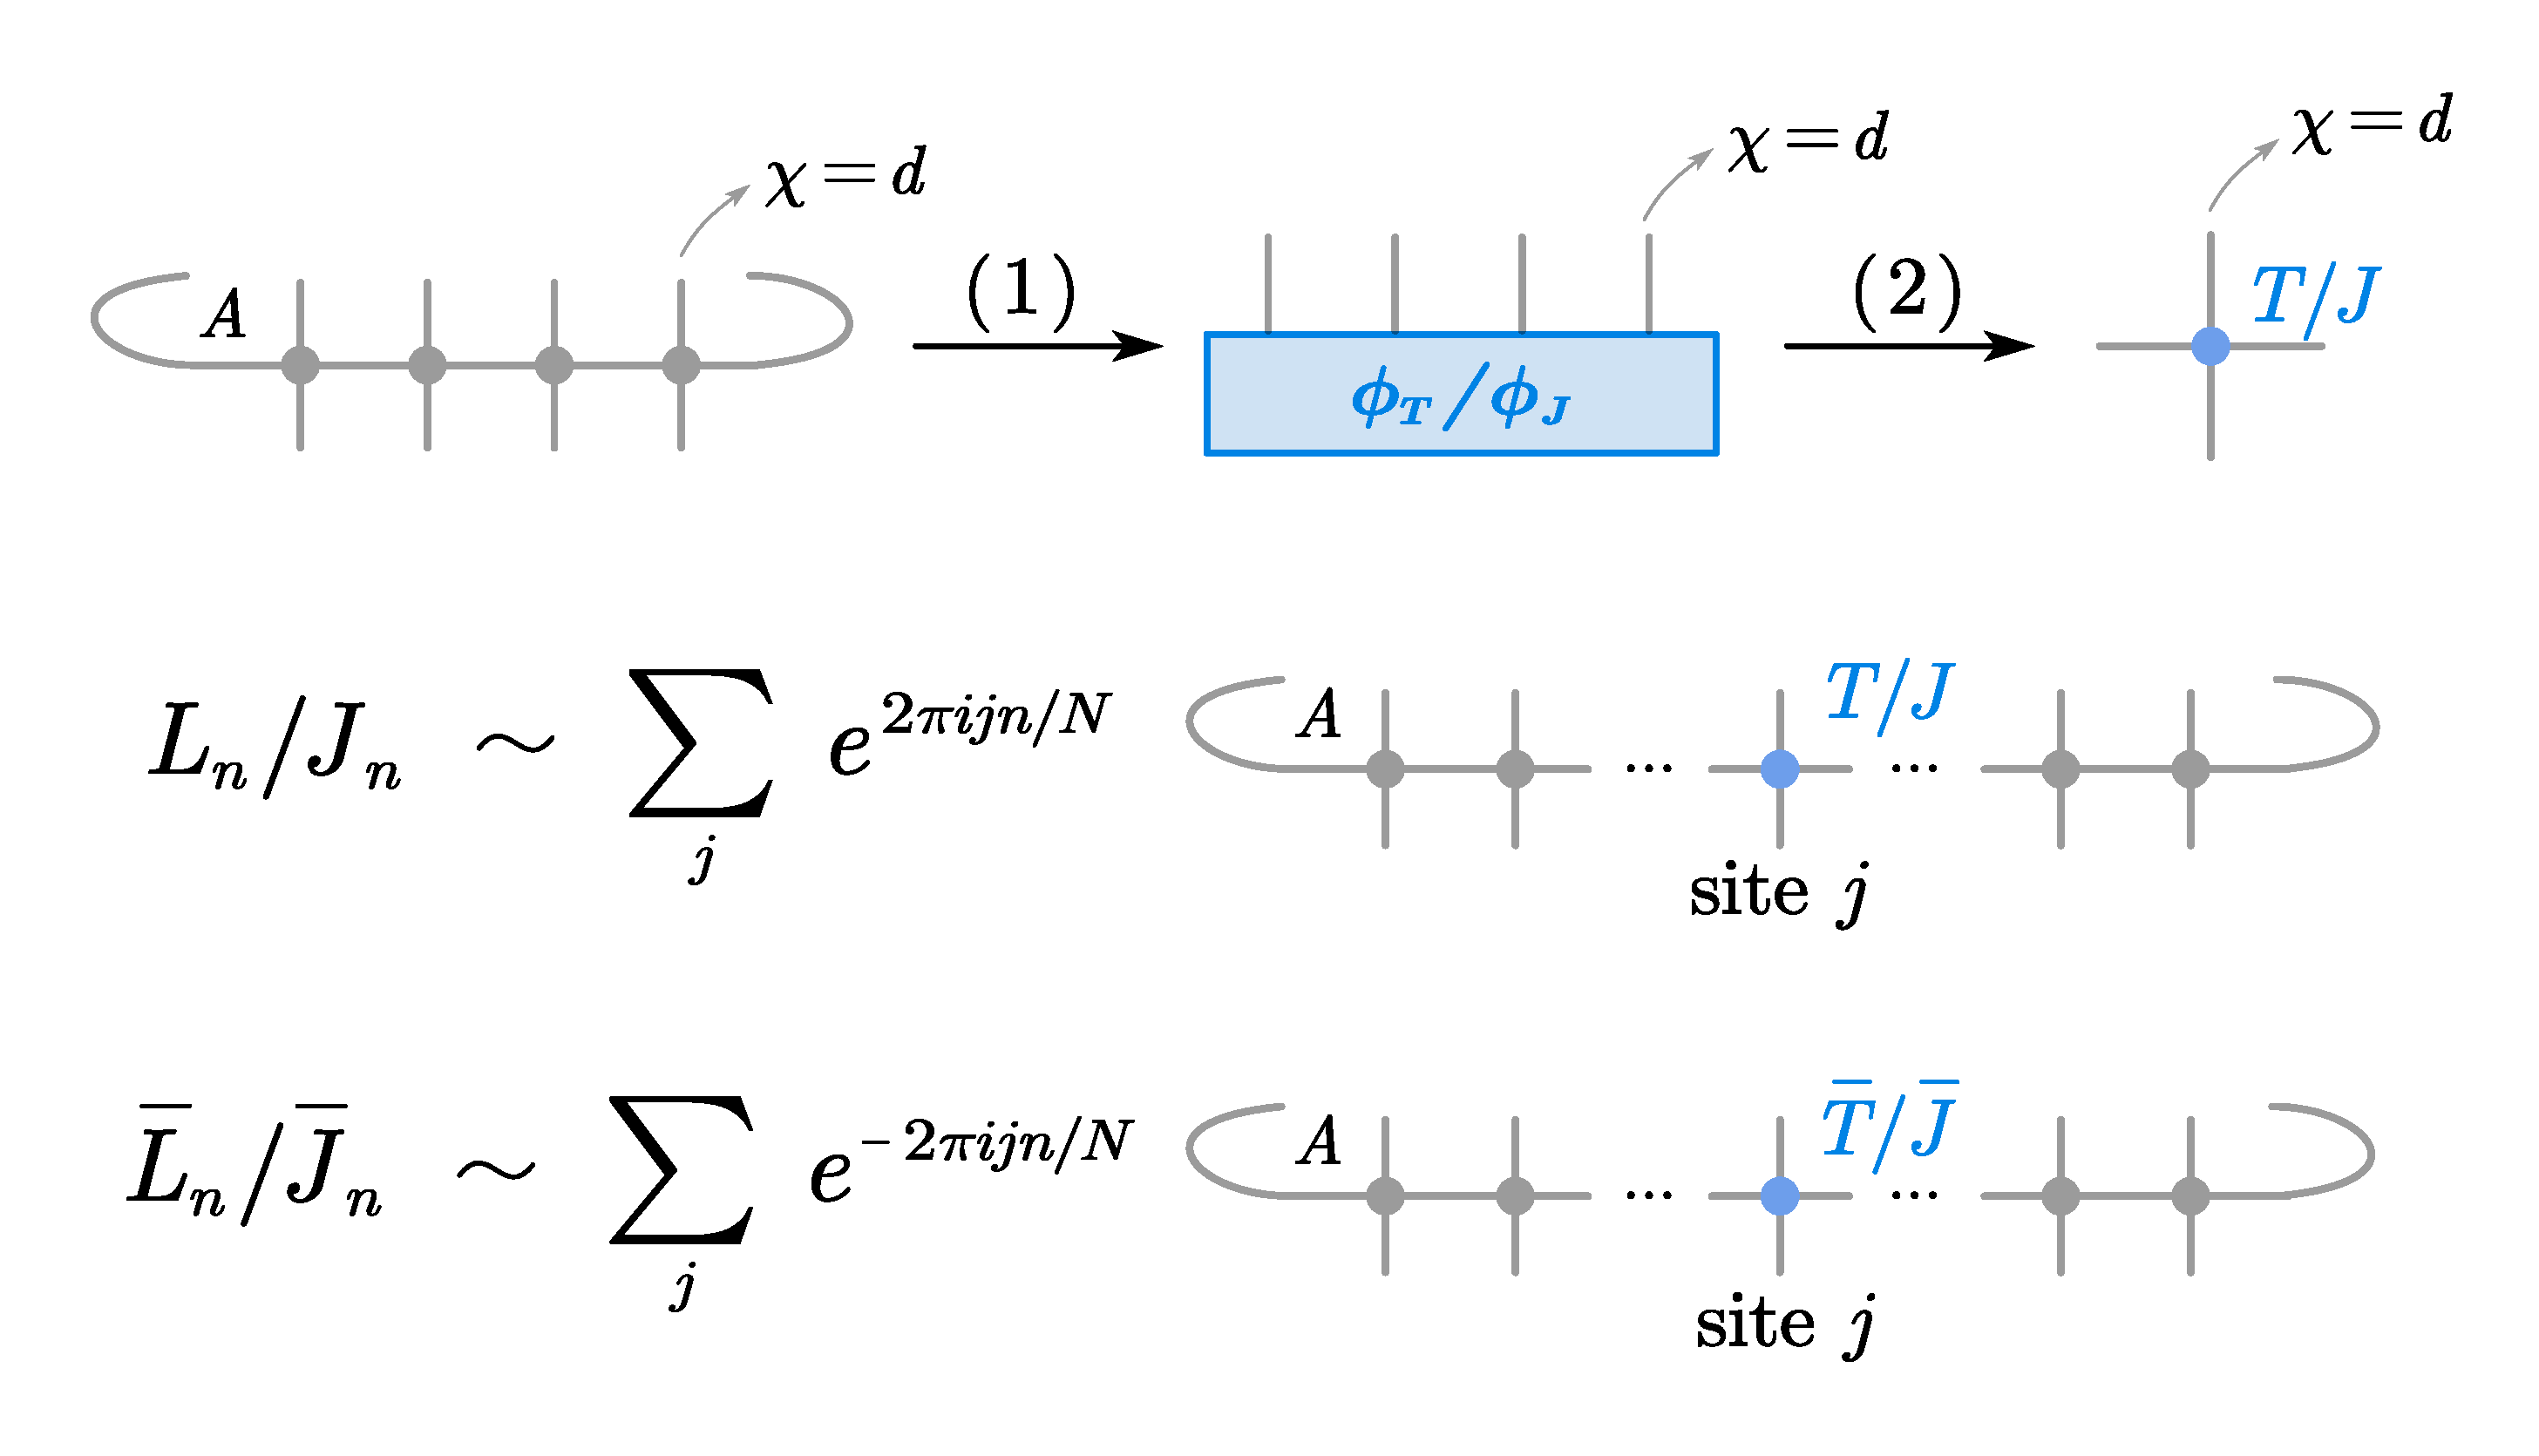
\includegraphics[width=0.9\textwidth]{images/virasoro/construction.pdf}

\end{columns}

\footnotetext{Image credit: \citet{wang2022virasoro}}

\end{frame}

\begin{frame}{Example: Virasoro algebra in Ising model}

\begin{columns}[T]

  \column{0.5\textwidth}

    \begin{itemize}
      \item Tensor unit:

        \begin{itemize}
          \item $A_{ijkl} = \ee^{-\beta (\sigma_i\sigma_j + \sigma_j\sigma_k + \sigma_k\sigma_l + \sigma_l\sigma_i)}$
          \item Use blocking or TRG/TNR
        \end{itemize}

      \item Can be verified by applying $L_n$ on cylinder eigenstates $\ket{\phi_\alpha}$ and checking $\langle\phi_\beta|L_n|\phi_\alpha\rangle$
      \item Numerical results:

        \begin{itemize}
          \item $N=8, \chi=4$ cylinder \\[1ex]
          \item $
              \frac{\lVert \langle\phi_\beta|L_n|\phi_\alpha\rangle \rVert}{\lVert \ket*{\phi_\beta} \rVert \cdot \lVert L_n\ket*{\phi_\alpha} \rVert} \gtrsim 0.9, \quad
              n=\pm1, \pm2.
            $
        \end{itemize}
    \end{itemize}

  \column{0.5\textwidth}

    \vspace{1em}
    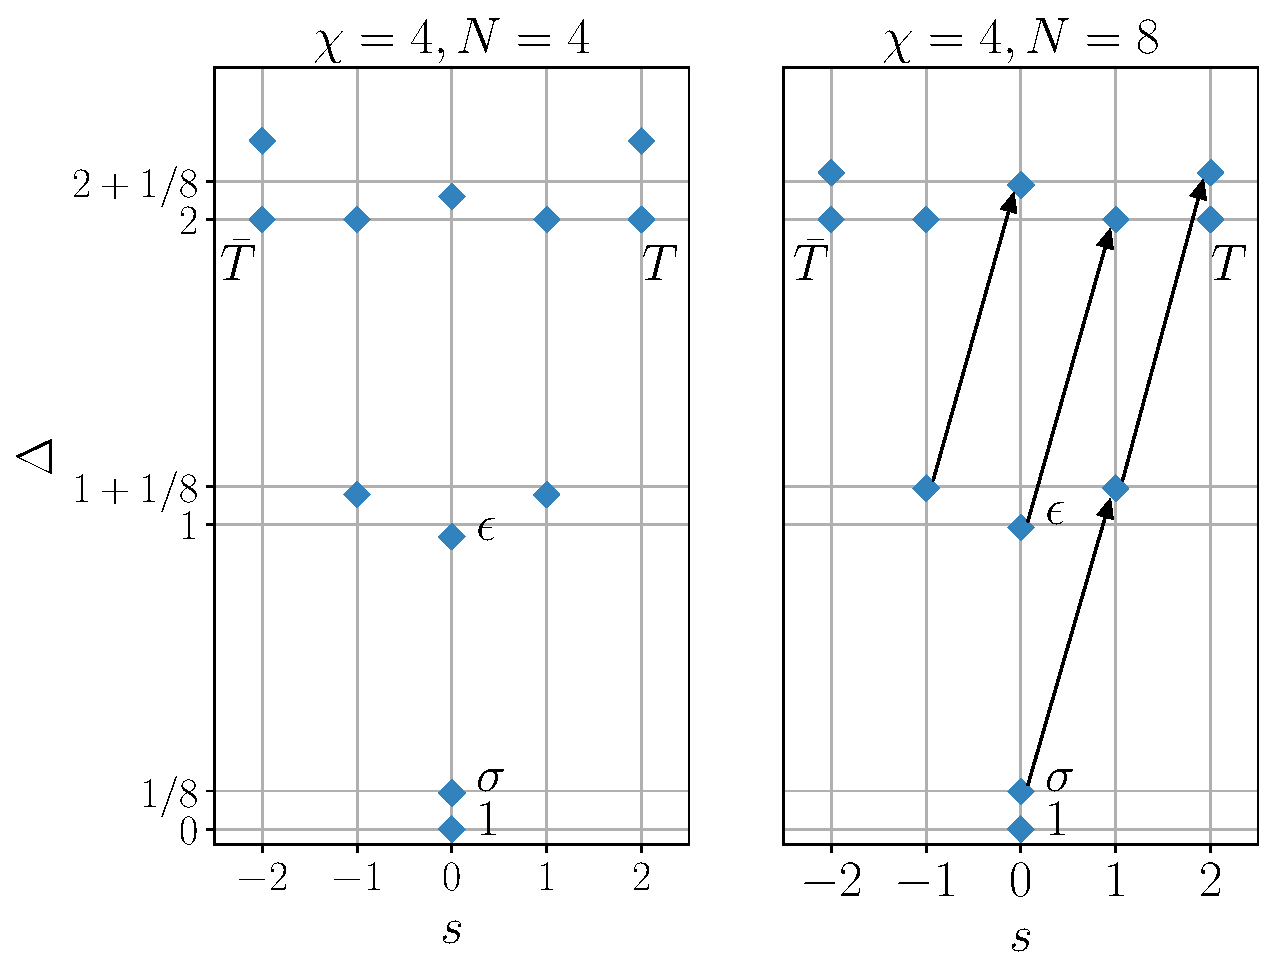
\includegraphics[width=\textwidth]{images/virasoro/ising-spectrum.pdf}

\end{columns}

\footnotetext{Image credit: \citet{wang2022virasoro}}

\end{frame}

\begin{frame}{Example: Kac--Moody algebra in dimer model}

\begin{columns}[T]

  \column{0.5\textwidth}

    \begin{itemize}
      \item Tensor unit:

        \begin{itemize}
          \item $B_{1111,2211,2121,1212,2222} = 1$
          \item $B_{1122} = 2$
        \end{itemize}

      \item Analysis of errors:

        \begin{itemize}
          \item Mixing of different Kac--Moody towers: lowest eigenstate is polluted by other primary states
          \item Mixing of lowering/raising actions within same towers: holomorphic and anti-holomorphic part are not fully separated
        \end{itemize}
    \end{itemize}

  \column{0.5\textwidth}

    \vspace{1em}
    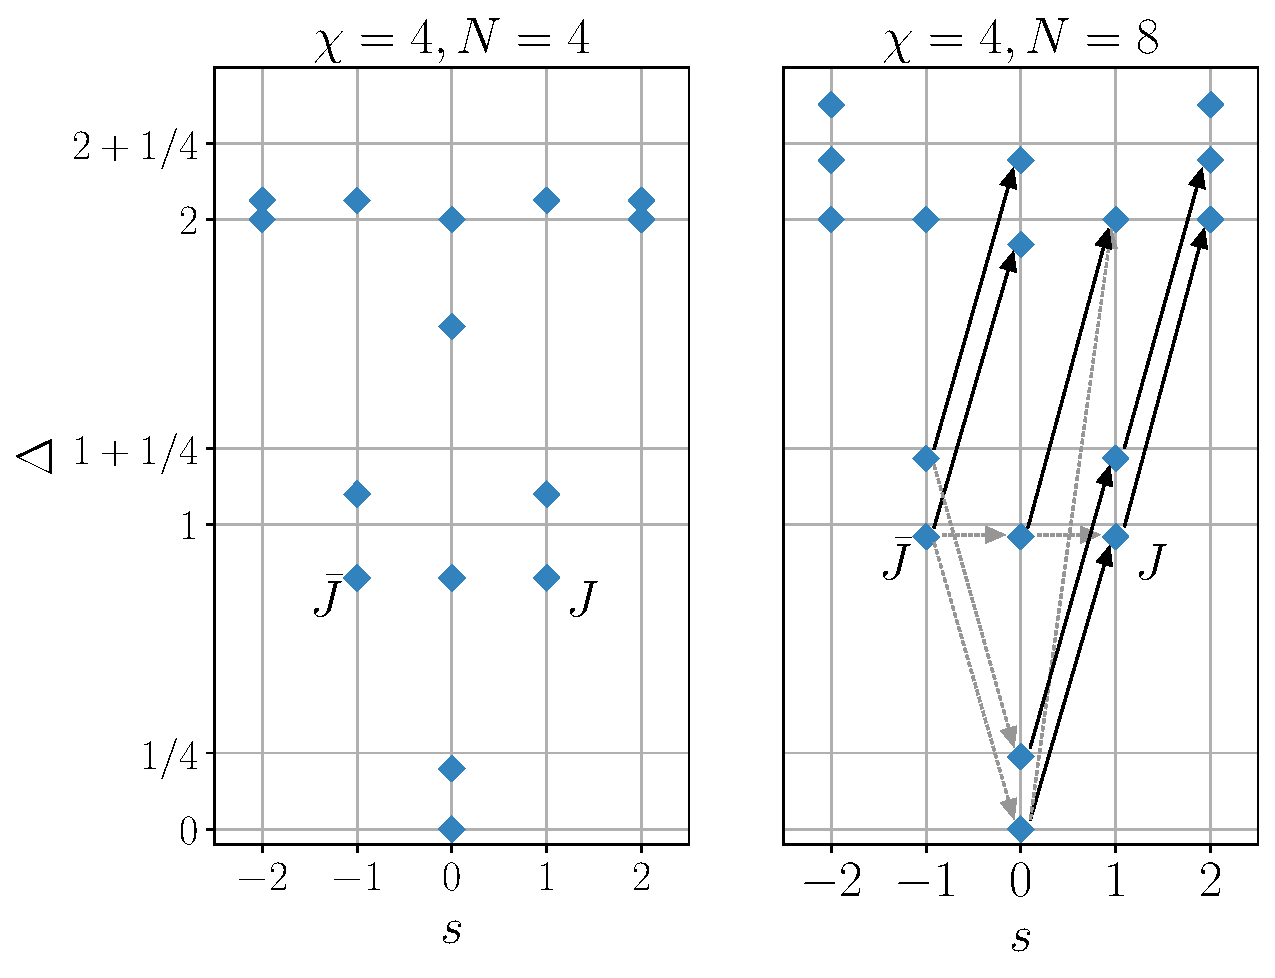
\includegraphics[width=\textwidth]{images/virasoro/dimer-spectrum.pdf}

\end{columns}

\footnotetext{Image credit: \citet{wang2022virasoro}}

\end{frame}

\begin{frame}{Fibonacci model: CFT spectrum}

\begin{columns}[T]

  \column{0.55\textwidth}

    \begin{itemize}
      \item Tensor unit and transfer matrix:

        \begin{itemize}
          \item
            \begingroup
              \tikzset{x=0.6em, y=0.6em, node font=\tiny}
              $
                  A_{ijkl}
                = \raisebox{0.4em}{\tikzinput{fibonacci/square-1}}
                = {\fontsize{0.6em}{1em}\selectfont \tikzinput{fibonacci/square-2}}
              $
            \endgroup
          \item
            \begingroup
              \tikzset{x=0.8em, y=0.8em, node font=\tiny}
              $\tilde{M}_{i_1 \cdots i_n, \, j_1 \cdots j_n} = \tikzinput{fibonacci/cylinder}$
            \endgroup
          \item Eliminate phases: $M = \tilde{M}\tilde{M}^\dagger$
        \end{itemize}

      \item Use matrix-free linear operator methods to solve the eigensystem
      \item Reduce level-crossing: assume $\Delta=A+B/n$ and optimize fitting results
    \end{itemize}

  \column{0.45\textwidth}

    \centering
    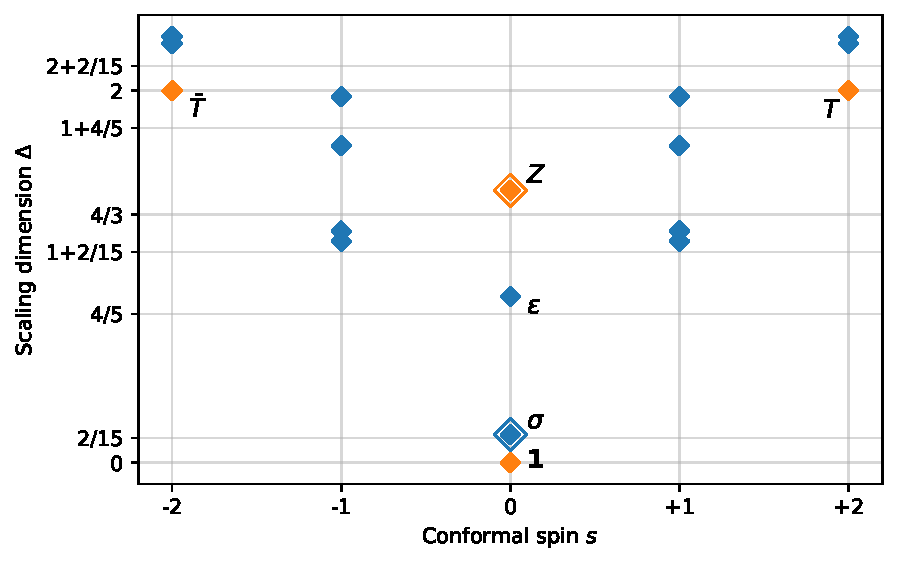
\includegraphics[width=0.85\textwidth]{images/fibonacci/fib-spectrum.pdf} \\[1ex]
    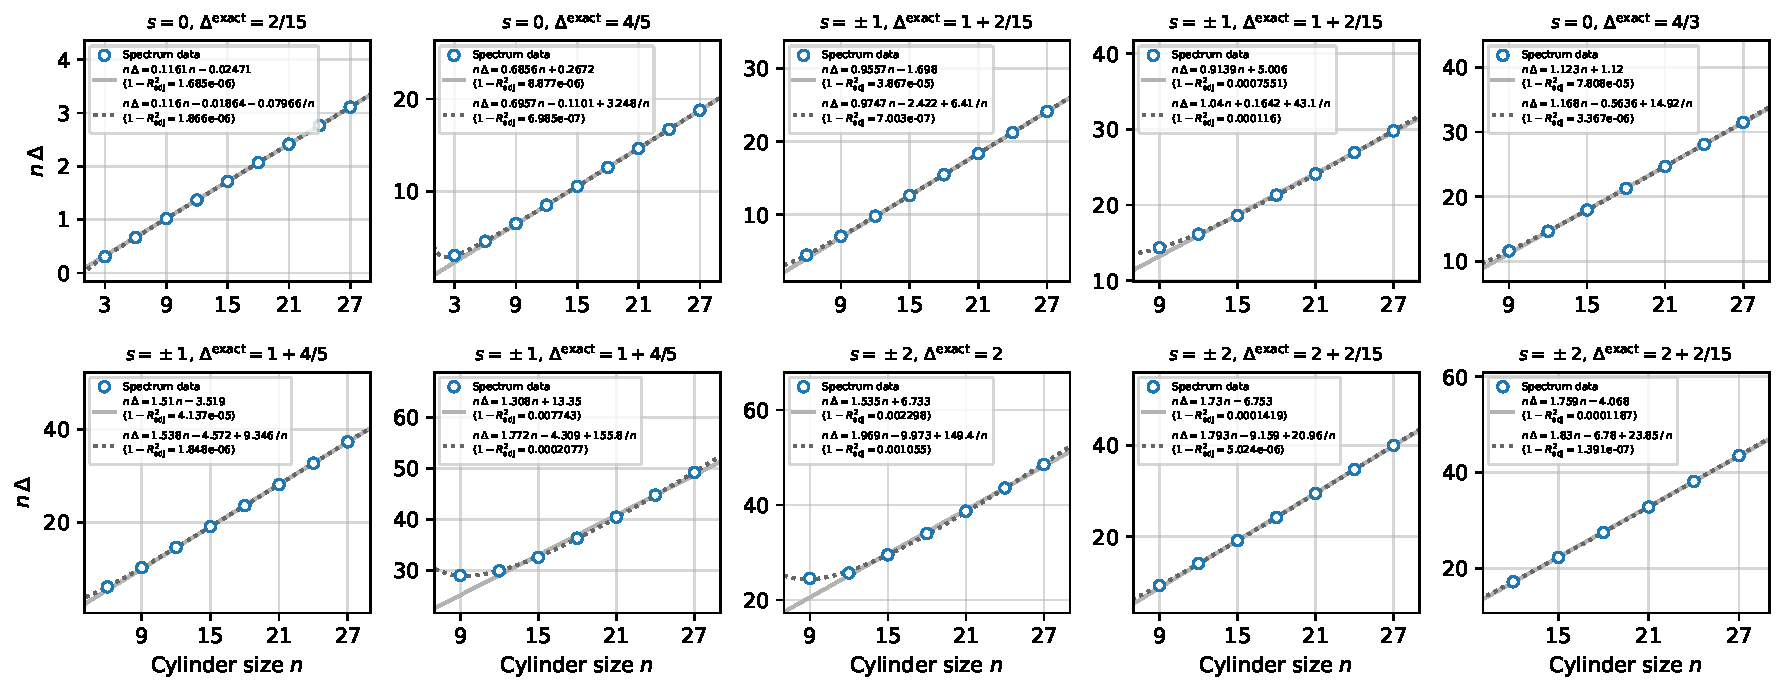
\includegraphics[width=0.95\textwidth]{images/fibonacci/fib-fitting.pdf}

\end{columns}

\footnotetext{Image credit: \citet{zeng2023virasoro}}

\end{frame}

\begin{frame}{Fibonacci model: topological projectors}

\begin{itemize}
  \item Project transfer matrix to certain topological sector of the CFT
  \item How to identify $T$:

    \begin{itemize}
      \item Descendant of the vacuum state \textrightarrow{} using the idempotent for trivial sector
    \end{itemize}

  \item Tensor network representation:

    \begingroup
      \scriptsize
      \tikzset{x=1em, y=1em, node font=\tiny}
      \begin{itemize}
        \item $
            \mathcal{P}_{\!1} = \frac{1}{\sqrt5}
            \left( \frac{1}{\phi} \, \mathcal{T}^{\,\1}_{\!\1\1} + \sqrt{\phi} \, \mathcal{T}^{\,\tau}_{\!\tau\1} \right), \enspace
            \mathcal{T}^{c}_{ab} = \raisebox{0.2em}{\tikzinput{tube-algebra-basis}}
          $
        \item $
              \raisebox{0.5em}{\tikzinput{idempotents-mpo-1}} \!\!
            = (d_\alpha d_\beta d_\gamma d_\delta)^{\frac14} G^{\beta i\gamma}_{j\alpha\delta}, \enspace
              \raisebox{0.5em}{\tikzinput{idempotents-mpo-2}} \!\!
            = (d_\alpha d_\beta d_\gamma d_\delta d_i d_j d_k)^{\frac14}
              G^{k\beta\delta}_{ij\alpha} G^{i\gamma\beta}_{kj\delta}
          $
        \item $
              G^{abc}_{ijk}
            = \frac{1}{\sqrt{d_j d_c}} \bigl[ F^{aik}_b \bigr]_{jc}
            = \frac{1}{\sqrt{d_a d_b d_c d_i d_j d_k}} \, \Tetrahedron jibcka
          $
      \end{itemize}
    \endgroup
\end{itemize}

\end{frame}

\begin{frame}{Fibonacci model: Virasoro algebra}

\begin{columns}[T]

  \column{0.55\textwidth}

    \begin{itemize}
      \item Reshape $T$:
        \begingroup
          \scriptsize
          \tikzset{x=1em, y=1em, node font=\tiny}
          $
            \begin{aligned}
              \tikzinput{fibonacci/padded-tensor-1} &= \tikzinput{fibonacci/padded-tensor-2} \\
              &\to \tikzinput{fibonacci/padded-tensor-3}
            \end{aligned}
          $
        \endgroup
      \item Cylinder size:

        \begin{itemize}
          \item Eigenstates: $n=18, \chi=2$
          \item Virasoro operators: $N=3, \chi=2^{n/3}$
        \end{itemize}
    \end{itemize}

  \column{0.45\textwidth}

    \vspace{1em}
    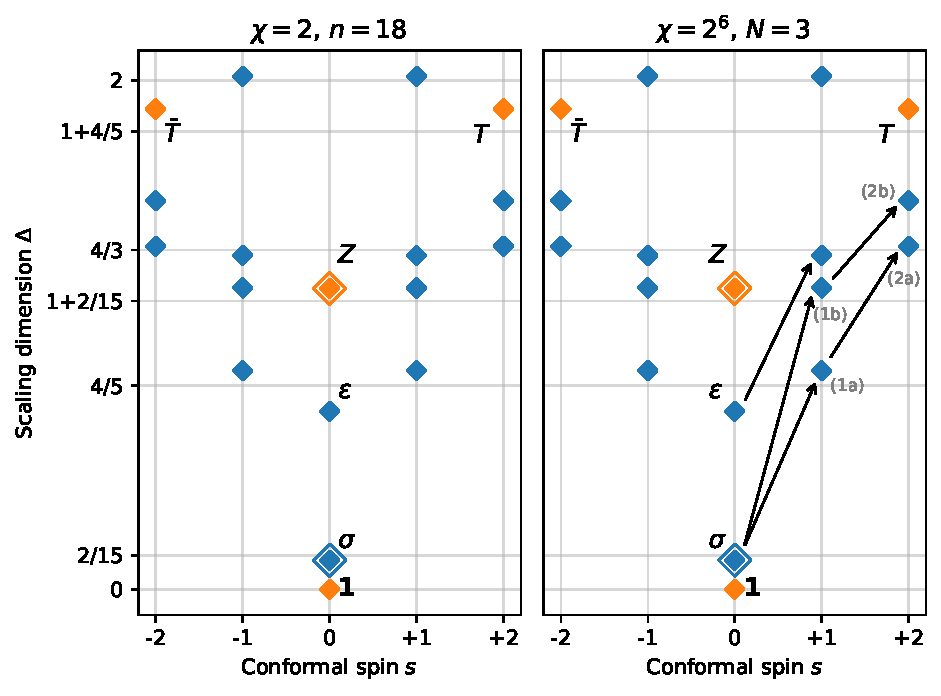
\includegraphics[width=\textwidth]{images/fibonacci/fib-virasoro.pdf}

\end{columns}

\end{frame}

\begin{frame}{Summary}

\begin{itemize}
  \item 
\end{itemize}

\end{frame}

\begin{frame}{References}
  \tiny
  \bibliography{main}
\end{frame}

\begingroup
  \setbeamercolor{background canvas}{bg=FudanBlue}
  \begin{frame}[plain]
    \vfill
    \begin{center}
      \color{white}
      \LARGE
      \textbf{Thank you!} \par
      \vspace{6em}
      \tiny
      \copyright{} 2023 Xiangdong Zeng
    \end{center}
    \vspace{-8em}
  \end{frame}
\endgroup

\end{document}
